\section{Breve historia del principio de acción: de Fermat a Feynman}

    Existe en la física una idea que reaparece, con ropajes distintos, en casi todos los niveles de descripción de la naturaleza: la idea de que el comportamiento efectivo de un sistema puede obtenerse exigiendo que cierta cantidad global, acumulada a lo largo de toda su historia, sea estacionaria. No se trata de una ley de fuerzas ni de una prescripción local sobre lo que ocurre en un instante, sino de una condición sobre la trayectoria completa, y esa diferencia de perspectiva, aparentemente solo estética, resultó ser el hilo conductor que llevó de la mecánica de Newton a la mecánica cuántica y de allí a la integral de camino que usaremos más adelante para describir la propagación de los fotones.

    El primer eco de esta idea es anterior en muchos siglos a la mecánica. Herón de Alejandría, en el siglo I de nuestra era, observó que un rayo de luz reflejado en un espejo plano recorre, entre dos puntos dados, el camino más corto de todos los que tocan la superficie, y esa observación permaneció como una curiosidad geométrica hasta que Pierre de Fermat, hacia 1662, la generalizó a la refracción sustituyendo la longitud geométrica por el tiempo de recorrido. La ley de Snell, que hasta entonces era un hecho experimental sin explicación, quedaba así deducida de un principio de economía: la luz escoge, entre todos los caminos concebibles, aquel para el cual el tiempo es estacionario. El resultado incomodó profundamente a sus contemporáneos, y la objeción que se le hizo es la misma que se repetirá en cada nueva encarnación del principio, a saber, que un criterio de este tipo parece atribuir a la luz el conocimiento anticipado de su destino, pues para escoger el camino óptimo habría que comparar todos los caminos posibles antes de recorrer ninguno.

    La traducción de esta idea al lenguaje de la mecánica fue obra de Pierre Louis Moreau de Maupertuis, quien en 1744 propuso su \textit{principio de mínima acción} definiendo la acción como la integral del producto de la masa por la velocidad y por el elemento de camino \citep{maupertuis1744accord}. La motivación de Maupertuis era en buena medida teológica, pues veía en la economía de la naturaleza una prueba de la sabiduría de su creador, y su formulación era tan vaga que resultaba difícil de aplicar a cualquier problema concreto; pero la intuición era correcta. Ese mismo año, y con una claridad matemática que Maupertuis nunca alcanzó, Leonhard Euler publicó el tratado en el que establece las condiciones que debe cumplir una curva para hacer estacionaria una integral \citep{euler1744methodus}, fundando de paso el cálculo de variaciones como disciplina. Euler demostró para el caso de una partícula sometida a fuerzas centrales que la trayectoria newtoniana es exactamente la que hace estacionaria la acción de Maupertuis, con lo cual el principio dejaba de ser una conjetura metafísica y pasaba a ser un teorema.

    El paso decisivo lo dio Joseph Louis Lagrange con la publicación de la \textit{Méchanique Analitique} en 1788 \citep{lagrange1788mecanique}, un libro del que su autor se enorgullecía de que no contuviera una sola figura. Lagrange comprendió que la verdadera ventaja del método variacional no reside en la economía de la naturaleza sino en la libertad de coordenadas: si las ecuaciones de movimiento se obtienen exigiendo que una integral escalar sea estacionaria, entonces tendrán la misma forma en cualquier sistema de coordenadas que se escoja, porque un escalar no sabe en qué coordenadas se le está evaluando. Las ligaduras, que en el lenguaje newtoniano obligan a introducir fuerzas de reacción desconocidas, desaparecen del problema sin más que escoger coordenadas adaptadas a ellas. Esa es la razón por la cual la mecánica lagrangiana se impuso, y no ninguna consideración sobre la economía del universo.

    Medio siglo más tarde William Rowan Hamilton, que había llegado a la mecánica desde la óptica, dio a la teoría su forma definitiva en dos memorias publicadas en 1834 y 1835 \citep{hamilton1834general, hamilton1835second}. Hamilton había demostrado en 1828 que todo sistema óptico puede describirse mediante una única función, la \textit{función característica}, cuyas derivadas parciales dan las direcciones de los rayos \citep{hamilton1828theory}, y al trasladar esa construcción a la mecánica descubrió que la misma estructura gobierna el movimiento de las partículas: existe una función de las coordenadas y del tiempo cuyas derivadas parciales son los momentos. La analogía es tan precisa que Hamilton la formuló explícitamente como un diccionario entre la óptica geométrica y la mecánica de partículas, con los frentes de onda correspondiendo a superficies de acción constante y los rayos a trayectorias. \textbf{Aquella analogía, que durante casi un siglo pareció una curiosidad formal sin contenido físico, resultó ser la pista que Schrödinger siguió en 1926 para construir la mecánica ondulatoria.} Carl Gustav Jacob Jacobi completó el programa poco después, mostrando que la función de Hamilton satisface una ecuación diferencial en derivadas parciales cuya solución completa resuelve por completo el problema mecánico \citep{jacobi1866vorlesungen}.

    El andamiaje algebraico que sostiene todo esto se había construido en paralelo. Siméon Denis Poisson había introducido en 1809 los corchetes que llevan su nombre al estudiar cómo varían las constantes de integración de un problema perturbado \citep{poisson1809memoire}, sin sospechar que estaba escribiendo la estructura algebraica que un siglo después Dirac reconocería como el límite clásico del conmutador cuántico. Joseph Liouville demostró en 1838 que el flujo generado por las ecuaciones de Hamilton conserva el volumen en el espacio de fase \citep{liouville1838note}, resultado que es el fundamento de la mecánica estadística. Y en 1918 Emmy Noether cerró el círculo conceptual al demostrar que toda simetría continua de la acción lleva asociada una cantidad conservada \citep{noether1918invariante}, convirtiendo las leyes de conservación, que hasta entonces eran hechos empíricos independientes, en consecuencias necesarias de la estructura del lagrangiano.

    La historia que nos interesa aquí, sin embargo, no termina en la mecánica clásica. En 1924 Louis de Broglie propuso que a toda partícula de momento $p$ le corresponde una longitud de onda $\lambda = h/p$ \citep{debroglie1924recherches}, y al hacerlo convirtió la analogía de Hamilton en una afirmación física: si la mecánica clásica es a la mecánica verdadera lo que la óptica geométrica es a la óptica ondulatoria, entonces debe existir una ecuación de ondas cuyo límite de longitud de onda corta reproduzca la ecuación de Hamilton-Jacobi. Erwin Schrödinger buscó esa ecuación durante el invierno de 1925 y la encontró en enero de 1926 \citep{schrodinger1926quantisierung}, y el camino que siguió, que reconstruiremos paso a paso en este capítulo, parte precisamente de la ecuación de Hamilton-Jacobi y de una sustitución exponencial. Siete años más tarde Paul Dirac observó que la amplitud de transición de la mecánica cuántica \textit{corresponde} a la exponencial de la acción clásica dividida por $\hbar$ \citep{dirac1933lagrangian}, y en 1948 Richard Feynman convirtió ese \textit{corresponde} en una igualdad, mostrando que la amplitud entre dos puntos es la suma de $e^{iS/\hbar}$ sobre todos los caminos que los unen \citep{feynman1948space}. Con ello la objeción que se le había hecho a Fermat tres siglos antes quedaba finalmente respondida: la luz no escoge un camino, los recorre todos, y el camino clásico es simplemente aquel en cuya vecindad las fases no se cancelan.

    Este capítulo recorre esa cadena en orden. Construiremos las ecuaciones de Lagrange desde la mecánica newtoniana, las obtendremos de nuevo a partir del principio de Hamilton, pasaremos al formalismo hamiltoniano mediante la transformada de Legendre, deduciremos la ecuación de Hamilton-Jacobi, la usaremos para llegar a la ecuación de Schrödinger siguiendo el razonamiento original, extenderemos el formalismo a sistemas continuos, que es lo que exige la cuantización del campo electromagnético del capítulo siguiente, y terminaremos con la integral de camino y con el propagador del oscilador armónico, que es la expresión de la que parte el capítulo dedicado a la propagación de los fotones.

\section{De Newton a Lagrange}

        La mecánica newtoniana describe un sistema de $N$ partículas mediante $N$ ecuaciones vectoriales
        \begin{equation}\label{eq:Newton}
            \dot{\mathbf{p}}_{i} = \mathbf{F}_{i}, \qquad \mathbf{p}_{i} = m_{i}\dot{\mathbf{r}}_{i}, \qquad i = 1,\ldots,N,
        \end{equation}
        lo que en coordenadas cartesianas equivale a $3N$ ecuaciones diferenciales de segundo orden. Si las fuerzas fuesen todas conocidas de antemano el problema estaría cerrado, pero en la práctica casi nunca lo están, porque los sistemas reales están sometidos a \textit{ligaduras}: la cuenta de un ábaco está obligada a permanecer sobre el alambre, las partículas de un sólido rígido mantienen fijas sus distancias mutuas, y la masa de un péndulo no puede alejarse del punto de suspensión más allá de la longitud del hilo. Las fuerzas que imponen estas condiciones, la reacción del alambre, las fuerzas internas del sólido, la tensión del hilo, no están dadas por ninguna ley constitutiva: son precisamente las que hacen falta, instante a instante, para que la condición se cumpla, de modo que son incógnitas del problema y no datos.

        Diremos que una ligadura es \textit{holónoma} cuando puede expresarse como una relación funcional entre las coordenadas y el tiempo,
        \begin{equation}\label{eq:Holonoma}
            f_{\alpha}(\mathbf{r}_{1},\mathbf{r}_{2},\ldots,\mathbf{r}_{N},t) = 0, \qquad \alpha = 1,\ldots,k,
        \end{equation}
        y \textit{no holónoma} en caso contrario, como ocurre con la condición de rodadura sin deslizamiento de una esfera sobre un plano, que involucra velocidades y no es integrable. Restringiremos en adelante el tratamiento al caso holónomo, que es el único que necesitaremos.

        La utilidad de \eqref{eq:Holonoma} es doble. Por una parte, cada una de las $k$ ligaduras elimina una coordenada independiente, de manera que el número de \textit{grados de libertad} del sistema pasa a ser
        \begin{equation}\label{eq:GradosLibertad}
            n = 3N - k .
        \end{equation}
        Por otra parte, y esto es lo esencial, las $k$ relaciones permiten introducir $n$ cantidades independientes $q_{1},\ldots,q_{n}$, las \textit{coordenadas generalizadas}, en términos de las cuales las posiciones quedan determinadas,
        \begin{equation}\label{eq:CoordGen}
            \mathbf{r}_{i} = \mathbf{r}_{i}(q_{1},q_{2},\ldots,q_{n},t), \qquad i = 1,\ldots,N .
        \end{equation}
        Las coordenadas generalizadas no tienen por qué ser longitudes: pueden ser ángulos, áreas, amplitudes de un modo normal o cualquier otro parámetro conveniente, y de hecho la libertad de escogerlas a conveniencia es lo que hace poderoso a todo el formalismo. En el capítulo siguiente veremos que las coordenadas generalizadas naturales del campo electromagnético en una cavidad son las amplitudes $q_{\mathbf{k},\lambda}(t)$ de sus modos normales, que no son posiciones de ninguna partícula.

        Nótese desde ahora que \eqref{eq:CoordGen} incorpora la ligadura de manera automática. Cualquier movimiento descrito por funciones $q_{j}(t)$ arbitrarias satisface \eqref{eq:Holonoma} idénticamente, porque las ligaduras ya fueron usadas al construir la parametrización. Las fuerzas de ligadura, que en el lenguaje newtoniano eran incógnitas adicionales, desaparecen del problema no porque se las haya calculado sino porque se ha escogido un lenguaje en el que no pueden ser nombradas.

        Para explotar esa idea necesitamos una noción de desplazamiento que respete las ligaduras. Llamaremos \textit{desplazamiento virtual} $\delta\mathbf{r}_{i}$ a un cambio infinitesimal de la configuración del sistema, compatible con las ligaduras, realizado a tiempo congelado. El adjetivo virtual indica que no se trata de un desplazamiento efectivamente recorrido durante la evolución, sino de una comparación imaginaria entre configuraciones simultáneas, y la congelación del tiempo es esencial: el desplazamiento real $d\mathbf{r}_{i}$ incluye el término $(\partial\mathbf{r}_{i}/\partial t)\,dt$ que proviene del movimiento de las propias ligaduras, mientras que el virtual no,
        \begin{equation}\label{eq:DespVirtual}
            \delta\mathbf{r}_{i} = \sum_{j=1}^{n}\frac{\partial\mathbf{r}_{i}}{\partial q_{j}}\,\delta q_{j},
            \qquad\text{frente a}\qquad
            d\mathbf{r}_{i} = \sum_{j=1}^{n}\frac{\partial\mathbf{r}_{i}}{\partial q_{j}}\,dq_{j} + \frac{\partial\mathbf{r}_{i}}{\partial t}\,dt .
        \end{equation}

        La hipótesis física que permite eliminar las fuerzas de ligadura es la siguiente, y hay que enunciarla con precisión porque todo lo demás descansa sobre ella.

        \begin{Assumption}\label{sup:TrabajoVirtual}
            El trabajo total realizado por las fuerzas de ligadura sobre cualquier desplazamiento virtual del sistema es nulo.
        \end{Assumption}

        El supuesto se cumple en todos los casos de interés práctico y su contenido geométrico es transparente: una fuerza de ligadura es perpendicular a la superficie sobre la cual obliga a moverse al sistema, y un desplazamiento virtual es tangente a esa superficie, de modo que su producto escalar se anula. La reacción normal de una mesa no realiza trabajo sobre un cuerpo que se desliza horizontalmente, la tensión de un hilo inextensible no realiza trabajo sobre la masa del péndulo porque es perpendicular al arco, y las fuerzas internas de un sólido rígido no realizan trabajo neto porque las distancias mutuas no cambian. El caso que queda excluido es el de la fricción de deslizamiento, que es antiparalela al desplazamiento y por tanto realiza trabajo negativo; los sistemas disipativos requieren un tratamiento aparte y no los consideraremos.

        Separamos entonces la fuerza sobre cada partícula en su parte aplicada y su parte de ligadura,
        \begin{equation}\label{eq:FuerzaSeparada}
            \mathbf{F}_{i} = \mathbf{F}_{i}^{(a)} + \mathbf{f}_{i},
        \end{equation}
        y escribamos la segunda ley \eqref{eq:Newton} en la forma en que d'Alembert la dispuso, pasando todo a un miembro,
        \begin{equation}\label{eq:dAlembertPartida}
            \mathbf{F}_{i}^{(a)} + \mathbf{f}_{i} - \dot{\mathbf{p}}_{i} = 0 .
        \end{equation}
        Multiplicando escalarmente por el desplazamiento virtual de la partícula $i$ y sumando sobre todas las partículas,
        \begin{equation}\label{eq:SumaVirtual}
            \sum_{i=1}^{N}\left(\mathbf{F}_{i}^{(a)} - \dot{\mathbf{p}}_{i}\right)\cdot\delta\mathbf{r}_{i}
            + \textcolor{red}{\sum_{i=1}^{N}\mathbf{f}_{i}\cdot\delta\mathbf{r}_{i}} = 0,
        \end{equation}
        donde el término marcado en rojo se anula en virtud del supuesto \ref{sup:TrabajoVirtual}. Queda así el \textit{principio de d'Alembert},
        \begin{equation}\label{eq:dAlembert}
            \sum_{i=1}^{N}\left(\mathbf{F}_{i}^{(a)} - \dot{\mathbf{p}}_{i}\right)\cdot\delta\mathbf{r}_{i} = 0,
        \end{equation}
        en el cual ya no aparece ninguna fuerza desconocida. El precio pagado es que \eqref{eq:dAlembert} no puede leerse componente a componente, porque los $\delta\mathbf{r}_{i}$ no son independientes entre sí: están ligados por \eqref{eq:Holonoma}. Ese es exactamente el problema que resuelven las coordenadas generalizadas, cuyas variaciones $\delta q_{j}$ sí son independientes por construcción.

        Vamos a traducir \eqref{eq:dAlembert} al lenguaje de las $q_{j}$. El primer término define las \textit{fuerzas generalizadas}: sustituyendo el desplazamiento virtual \eqref{eq:DespVirtual} e intercambiando el orden de las sumas,
        \begin{equation}\label{eq:FuerzaGen}
            \sum_{i=1}^{N}\mathbf{F}_{i}^{(a)}\cdot\delta\mathbf{r}_{i}
            = \sum_{i=1}^{N}\sum_{j=1}^{n}\mathbf{F}_{i}^{(a)}\cdot\frac{\partial\mathbf{r}_{i}}{\partial q_{j}}\,\delta q_{j}
            \equiv \sum_{j=1}^{n} Q_{j}\,\delta q_{j},
            \qquad
            Q_{j} \equiv \sum_{i=1}^{N}\mathbf{F}_{i}^{(a)}\cdot\frac{\partial\mathbf{r}_{i}}{\partial q_{j}} .
        \end{equation}
        Adviértase que $Q_{j}$ no tiene por qué tener dimensiones de fuerza; si $q_{j}$ es un ángulo, entonces $Q_{j}$ es un torque. Lo único que la definición garantiza es que el producto $Q_{j}\delta q_{j}$ tenga dimensiones de trabajo, que es lo que exige la consistencia de \eqref{eq:FuerzaGen}.

        El segundo término requiere más cuidado, y lo trabajaremos en detalle porque de él sale toda la estructura. Partimos de
        \begin{equation}\label{eq:TerminoInercial}
            \sum_{i=1}^{N}\dot{\mathbf{p}}_{i}\cdot\delta\mathbf{r}_{i}
            = \sum_{i=1}^{N}\sum_{j=1}^{n} m_{i}\ddot{\mathbf{r}}_{i}\cdot\frac{\partial\mathbf{r}_{i}}{\partial q_{j}}\,\delta q_{j},
        \end{equation}
        y observamos que el sumando admite reescribirse como la derivada temporal de un producto menos el término que sobra, que es la regla del producto leída al revés,
        \begin{equation}\label{eq:ReglaProductoInversa}
            m_{i}\ddot{\mathbf{r}}_{i}\cdot\frac{\partial\mathbf{r}_{i}}{\partial q_{j}}
            = \frac{d}{dt}\left(m_{i}\dot{\mathbf{r}}_{i}\cdot\frac{\partial\mathbf{r}_{i}}{\partial q_{j}}\right)
            - m_{i}\dot{\mathbf{r}}_{i}\cdot\frac{d}{dt}\left(\frac{\partial\mathbf{r}_{i}}{\partial q_{j}}\right).
        \end{equation}
        El paso se justifica porque el primer término de la derecha, al derivarse, produce el término de la izquierda más el segundo término de la derecha con signo contrario, de modo que la identidad es exacta y no una aproximación.

        Necesitamos ahora dos identidades auxiliares, y las demostramos por separado porque son el verdadero contenido técnico de la deducción. La primera relaciona la derivada de la posición respecto de una coordenada generalizada con la derivada de la velocidad respecto de la velocidad generalizada. Derivando \eqref{eq:CoordGen} respecto del tiempo mediante la regla de la cadena,
        \begin{equation}\label{eq:VelocidadCadena}
            \mathbf{v}_{i} \equiv \dot{\mathbf{r}}_{i} = \sum_{l=1}^{n}\frac{\partial\mathbf{r}_{i}}{\partial q_{l}}\dot{q}_{l} + \frac{\partial\mathbf{r}_{i}}{\partial t},
        \end{equation}
        y derivando esta expresión respecto de $\dot{q}_{j}$ notamos que las funciones $\partial\mathbf{r}_{i}/\partial q_{l}$ y $\partial\mathbf{r}_{i}/\partial t$ dependen solamente de las coordenadas y del tiempo, nunca de las velocidades, de manera que se comportan como constantes en esa derivación y solo sobrevive el término $l = j$,
        \begin{equation}\label{eq:CancelacionPuntos}
            \frac{\partial\mathbf{v}_{i}}{\partial\dot{q}_{j}}
            = \sum_{l=1}^{n}\frac{\partial\mathbf{r}_{i}}{\partial q_{l}}\,\frac{\partial\dot{q}_{l}}{\partial\dot{q}_{j}}
            + \textcolor{red}{\frac{\partial}{\partial\dot{q}_{j}}\frac{\partial\mathbf{r}_{i}}{\partial t}}
            = \sum_{l=1}^{n}\frac{\partial\mathbf{r}_{i}}{\partial q_{l}}\,\delta_{lj}
            = \frac{\partial\mathbf{r}_{i}}{\partial q_{j}} .
        \end{equation}
        Esta identidad, conocida como \textit{cancelación de los puntos}, dice que en lo que respecta a la derivación las velocidades generalizadas entran linealmente en las velocidades cartesianas con coeficientes que son exactamente los vectores tangentes a la superficie de configuración.

        La segunda identidad afirma que la derivada temporal total y la derivada parcial respecto de $q_{j}$ conmutan cuando actúan sobre la posición. Calculando explícitamente el miembro izquierdo mediante la regla de la cadena,
        \begin{equation}\label{eq:ConmutanDerivadas}
            \frac{d}{dt}\left(\frac{\partial\mathbf{r}_{i}}{\partial q_{j}}\right)
            = \sum_{l=1}^{n}\frac{\partial^{2}\mathbf{r}_{i}}{\partial q_{l}\partial q_{j}}\dot{q}_{l}
            + \frac{\partial^{2}\mathbf{r}_{i}}{\partial t\,\partial q_{j}}
            = \frac{\partial}{\partial q_{j}}\left(\sum_{l=1}^{n}\frac{\partial\mathbf{r}_{i}}{\partial q_{l}}\dot{q}_{l} + \frac{\partial\mathbf{r}_{i}}{\partial t}\right)
            = \frac{\partial\mathbf{v}_{i}}{\partial q_{j}},
        \end{equation}
        donde hemos usado la igualdad de las derivadas parciales cruzadas, válida porque las funciones $\mathbf{r}_{i}$ son de clase $C^{2}$, y el hecho de que $\dot{q}_{l}$ no depende de $q_{j}$, lo que permite introducir la derivada parcial dentro de la suma.

        Sustituyendo \eqref{eq:CancelacionPuntos} y \eqref{eq:ConmutanDerivadas} en \eqref{eq:ReglaProductoInversa} obtenemos
        \begin{equation}\label{eq:TerminoInercial2}
            m_{i}\ddot{\mathbf{r}}_{i}\cdot\frac{\partial\mathbf{r}_{i}}{\partial q_{j}}
            = \frac{d}{dt}\left(m_{i}\mathbf{v}_{i}\cdot\frac{\partial\mathbf{v}_{i}}{\partial\dot{q}_{j}}\right)
            - m_{i}\mathbf{v}_{i}\cdot\frac{\partial\mathbf{v}_{i}}{\partial q_{j}},
        \end{equation}
        y ambos términos son ahora derivadas de una misma cantidad escalar. En efecto, usando que
        \begin{equation}\label{eq:DerivadaCuadrado}
            \frac{\partial}{\partial\dot{q}_{j}}\left(\frac{1}{2}m_{i}v_{i}^{2}\right) = m_{i}\mathbf{v}_{i}\cdot\frac{\partial\mathbf{v}_{i}}{\partial\dot{q}_{j}},
            \qquad
            \frac{\partial}{\partial q_{j}}\left(\frac{1}{2}m_{i}v_{i}^{2}\right) = m_{i}\mathbf{v}_{i}\cdot\frac{\partial\mathbf{v}_{i}}{\partial q_{j}},
        \end{equation}
        y sumando sobre todas las partículas, aparece la energía cinética total
        \begin{equation}\label{eq:EnergiaCinetica}
            T = \sum_{i=1}^{N}\frac{1}{2}m_{i}v_{i}^{2},
        \end{equation}
        de modo que \eqref{eq:TerminoInercial} se convierte en
        \begin{equation}\label{eq:TerminoInercial3}
            \sum_{i=1}^{N}\dot{\mathbf{p}}_{i}\cdot\delta\mathbf{r}_{i}
            = \sum_{j=1}^{n}\left[\frac{d}{dt}\left(\frac{\partial T}{\partial\dot{q}_{j}}\right) - \frac{\partial T}{\partial q_{j}}\right]\delta q_{j} .
        \end{equation}

        Llevando \eqref{eq:FuerzaGen} y \eqref{eq:TerminoInercial3} al principio de d'Alembert \eqref{eq:dAlembert} resulta
        \begin{equation}\label{eq:dAlembertGen}
            \sum_{j=1}^{n}\left[\frac{d}{dt}\left(\frac{\partial T}{\partial\dot{q}_{j}}\right) - \frac{\partial T}{\partial q_{j}} - Q_{j}\right]\delta q_{j} = 0 .
        \end{equation}
        Aquí sí podemos leer la ecuación componente a componente, y esta es la ganancia de todo el rodeo: como las coordenadas generalizadas son independientes, las variaciones $\delta q_{j}$ pueden escogerse arbitrariamente y una a una, de manera que escogiendo $\delta q_{1}\neq 0$ con todas las demás nulas se concluye que el corchete correspondiente a $j=1$ se anula, y repitiendo el argumento para cada índice,
        \begin{equation}\label{eq:LagrangeT}
            \frac{d}{dt}\left(\frac{\partial T}{\partial\dot{q}_{j}}\right) - \frac{\partial T}{\partial q_{j}} = Q_{j}, \qquad j = 1,\ldots,n .
        \end{equation}

        Falta un último paso para llegar a la forma canónica. Supongamos que las fuerzas aplicadas derivan de un potencial escalar $V(\mathbf{r}_{1},\ldots,\mathbf{r}_{N},t)$, es decir $\mathbf{F}_{i}^{(a)} = -\nabla_{i}V$. Entonces, por la definición \eqref{eq:FuerzaGen} y la regla de la cadena,
        \begin{equation}\label{eq:FuerzaGenPotencial}
            Q_{j} = -\sum_{i=1}^{N}\nabla_{i}V\cdot\frac{\partial\mathbf{r}_{i}}{\partial q_{j}} = -\frac{\partial V}{\partial q_{j}},
        \end{equation}
        y sustituyendo en \eqref{eq:LagrangeT} y agrupando todo en un miembro,
        \begin{equation}\label{eq:LagrangePaso}
            \frac{d}{dt}\left(\frac{\partial T}{\partial\dot{q}_{j}}\right) - \frac{\partial (T-V)}{\partial q_{j}} = 0 .
        \end{equation}
        Como el potencial no depende de las velocidades, se cumple $\partial V/\partial\dot{q}_{j} = 0$ y por tanto podemos sumar ese cero dentro de la derivada temporal sin alterar nada,
        \begin{equation}\label{eq:SumaCero}
            \frac{\partial T}{\partial\dot{q}_{j}} = \frac{\partial T}{\partial\dot{q}_{j}} - \textcolor{blue}{\frac{\partial V}{\partial\dot{q}_{j}}} = \frac{\partial(T-V)}{\partial\dot{q}_{j}},
        \end{equation}
        donde el término en azul se ha introducido deliberadamente porque vale cero. Definiendo la \textit{función lagrangiana}
        \begin{equation}\label{eq:Lagrangiano}
            L(q,\dot{q},t) \equiv T - V,
        \end{equation}
        las dos derivadas quedan referidas a un mismo objeto y obtenemos las \textit{ecuaciones de Lagrange}
        \begin{equation}\label{eq:EulerLagrange}
            \boxed{\;\frac{d}{dt}\left(\frac{\partial L}{\partial\dot{q}_{j}}\right) - \frac{\partial L}{\partial q_{j}} = 0, \qquad j = 1,\ldots,n .\;}
        \end{equation}

        Lo que se ha conseguido es mucho más de lo que sugiere el aspecto inocente de \eqref{eq:EulerLagrange}. Hemos pasado de $3N$ ecuaciones vectoriales acopladas, con $k$ fuerzas de ligadura desconocidas, a $n = 3N-k$ ecuaciones escalares sin incógnitas espurias, y toda la dinámica del sistema está codificada en una única función escalar $L$. La diferencia $T-V$ no tiene, hay que decirlo, ninguna interpretación física directa: no es una energía que se conserve ni una cantidad que se mida en el laboratorio, y el intento de dotarla de significado intuitivo ha producido más confusión que claridad. Su importancia es estructural y no sustancial: es la función cuya estacionariedad reproduce las ecuaciones de movimiento, y eso basta. La justificación profunda de por qué debe ser precisamente $T-V$ y no otra combinación la daremos en la sección siguiente, donde las mismas ecuaciones surgirán de un principio variacional que no presupone las leyes de Newton.

\section{El principio de Hamilton y el cálculo de variaciones}

        La deducción anterior partió de las leyes de Newton y llegó a las ecuaciones de Lagrange. Vamos a invertir ahora el orden lógico, postulando un principio integral del que las ecuaciones de movimiento se deduzcan, porque esa formulación es la que se generaliza sin cambios a los campos, a la relatividad y a la teoría cuántica, mientras que la segunda ley de Newton no lo hace.

        Consideremos un sistema de $n$ grados de libertad y fijemos dos configuraciones, la inicial $q(t_{1}) = q^{(1)}$ y la final $q(t_{2}) = q^{(2)}$. Llamaremos \textit{camino} a cualquier función $q(t)$ suficientemente suave que una ambas configuraciones en el intervalo dado, sin exigirle que satisfaga las ecuaciones de movimiento; la inmensa mayoría de los caminos así definidos son físicamente imposibles, y eso es intencional.

        \begin{myDef}\label{def:Accion}
            Se llama \textit{acción} del sistema al funcional que a cada camino $q(t)$ le asigna el número real
            \begin{equation}\label{eq:Accion}
                S[q] = \int_{t_{1}}^{t_{2}} L\left(q(t),\dot{q}(t),t\right)\,dt .
            \end{equation}
        \end{myDef}

        La acción no es una función de un número sino de una función entera, razón por la cual se la llama funcional y se escribe con corchetes. Sus dimensiones son las de energía por tiempo, que son también las de momento por longitud y las de momento angular; que $\hbar$ tenga precisamente esas dimensiones no es una coincidencia sino la primera señal de que la acción es la cantidad que mide, en unidades cuánticas, cuán clásico es un sistema.

        El principio que sustituye a las leyes de Newton es el siguiente.

        \begin{Assumption}[Principio de Hamilton]\label{sup:Hamilton}
            El movimiento efectivo del sistema entre dos configuraciones fijas es aquel para el cual la acción \eqref{eq:Accion} es estacionaria frente a variaciones infinitesimales del camino que dejan fijos los extremos.
        \end{Assumption}

        Hay que insistir en la palabra estacionaria y no mínima, pese a que el principio se llame tradicionalmente de mínima acción. Para tiempos suficientemente cortos el camino clásico efectivamente minimiza la acción, pero para tiempos largos puede tratarse de un punto silla, y el ejemplo estándar es el del oscilador armónico más allá de medio período. Lo que la física exige es que la primera variación se anule, no que el valor sea el menor posible.

        Para dar contenido operativo al supuesto \ref{sup:Hamilton} hay que definir qué significa variar un camino. Introducimos, como en la figura \ref{fig:VariacionCamino}, una familia uniparamétrica de caminos
        \begin{equation}\label{eq:FamiliaCaminos}
            q_{j}(t,\varepsilon) = q_{j}(t,0) + \varepsilon\,\eta_{j}(t),
        \end{equation}
        donde $q_{j}(t,0)$ es el camino sobre el cual queremos evaluar la estacionariedad, $\varepsilon$ es un parámetro real infinitesimal y las funciones $\eta_{j}(t)$ son arbitrarias salvo por dos condiciones: deben ser derivables y deben anularse en los extremos,
        \begin{equation}\label{eq:ExtremosFijos}
            \eta_{j}(t_{1}) = \eta_{j}(t_{2}) = 0, \qquad j = 1,\ldots,n,
        \end{equation}
        que es la traducción matemática de que todos los caminos de la familia parten de la misma configuración inicial y llegan a la misma configuración final. Derivando \eqref{eq:FamiliaCaminos} respecto del tiempo, la variación de la velocidad resulta ser la derivada de la variación,
        \begin{equation}\label{eq:VariacionVelocidad}
            \dot{q}_{j}(t,\varepsilon) = \dot{q}_{j}(t,0) + \varepsilon\,\dot{\eta}_{j}(t),
            \qquad\text{es decir}\qquad
            \delta\dot{q}_{j} = \frac{d}{dt}\,\delta q_{j},
        \end{equation}
        propiedad que usaremos de inmediato y que es cierta porque la variación se toma a tiempo fijo mientras que la derivada se toma a $\varepsilon$ fijo, de modo que ambas operaciones conmutan.

        Sobre esta familia la acción se convierte en una función ordinaria del parámetro,
        \begin{equation}\label{eq:AccionEpsilon}
            S(\varepsilon) = \int_{t_{1}}^{t_{2}} L\left(q(t,\varepsilon),\dot{q}(t,\varepsilon),t\right)dt,
        \end{equation}
        y la condición de estacionariedad se reduce a la condición de que la derivada ordinaria de $S(\varepsilon)$ se anule en $\varepsilon = 0$ para toda elección de las funciones $\eta_{j}$. Definimos por ello la \textit{primera variación} de la acción como
        \begin{equation}\label{eq:PrimeraVariacion}
            \delta S \equiv \left.\frac{dS}{d\varepsilon}\right|_{\varepsilon=0}\varepsilon .
        \end{equation}

        \begin{figure}[htbp]
            \centering
            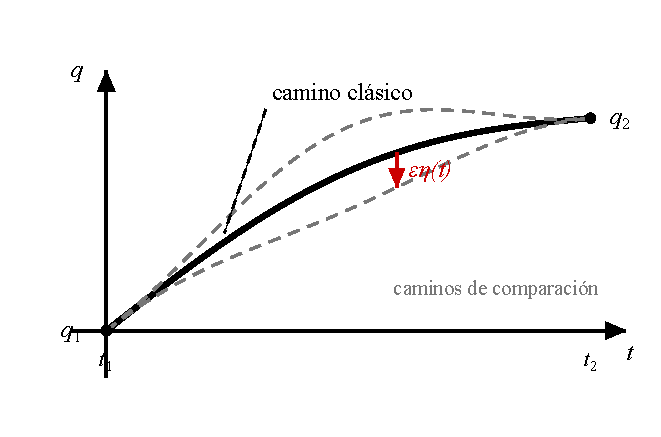
\includegraphics[width=0.62\linewidth]{Capitulo 3/Figuras/VariacionCamino.pdf}
            \caption{El camino efectivo y los caminos de comparación que se usan para variarlo. Todos parten de la misma configuración inicial y llegan a la misma final, de modo que la desviación $\varepsilon\eta(t)$ se anula en los dos extremos.}
            \label{fig:VariacionCamino}
        \end{figure}

        Podemos calcular esa derivada explícitamente. Derivando bajo el signo integral, lo que es lícito porque el integrando es continuo junto con su derivada respecto de $\varepsilon$ en un intervalo compacto, y aplicando la regla de la cadena,
        \begin{equation}\label{eq:DerivadaAccion}
            \frac{dS}{d\varepsilon} = \int_{t_{1}}^{t_{2}}\sum_{j=1}^{n}\left[\frac{\partial L}{\partial q_{j}}\frac{\partial q_{j}}{\partial\varepsilon} + \frac{\partial L}{\partial\dot{q}_{j}}\frac{\partial\dot{q}_{j}}{\partial\varepsilon}\right]dt
            = \int_{t_{1}}^{t_{2}}\sum_{j=1}^{n}\left[\frac{\partial L}{\partial q_{j}}\eta_{j} + \frac{\partial L}{\partial\dot{q}_{j}}\dot{\eta}_{j}\right]dt,
        \end{equation}
        donde el término $\partial L/\partial t$ no aparece porque el tiempo no depende de $\varepsilon$.

        El obstáculo es que en \eqref{eq:DerivadaAccion} figuran tanto $\eta_{j}$ como $\dot{\eta}_{j}$, y mientras eso sea así no podremos concluir nada sobre el corchete, porque una función y su derivada no son independientes. El recurso es integrar por partes el segundo término para transferir la derivada de $\eta_{j}$ hacia el otro factor. Escribiendo la regla del producto al revés,
        \begin{equation}\label{eq:ParaPartes}
            \frac{\partial L}{\partial\dot{q}_{j}}\dot{\eta}_{j}
            = \frac{d}{dt}\left(\frac{\partial L}{\partial\dot{q}_{j}}\,\eta_{j}\right) - \frac{d}{dt}\left(\frac{\partial L}{\partial\dot{q}_{j}}\right)\eta_{j},
        \end{equation}
        e integrando entre los dos instantes, el primer término de la derecha es una derivada total y produce una contribución de frontera,
        \begin{equation}\label{eq:TerminoFrontera}
            \int_{t_{1}}^{t_{2}}\frac{d}{dt}\left(\frac{\partial L}{\partial\dot{q}_{j}}\,\eta_{j}\right)dt
            = \textcolor{red}{\left.\frac{\partial L}{\partial\dot{q}_{j}}\,\eta_{j}\right|_{t_{1}}^{t_{2}}} = 0,
        \end{equation}
        que se anula porque las $\eta_{j}$ se anulan en ambos extremos según \eqref{eq:ExtremosFijos}. Este es el lugar preciso en el que la condición de extremos fijos hace su trabajo, y vale la pena retenerlo, porque cuando más adelante permitamos que el extremo final se mueva, ese mismo término de frontera dejará de anularse y será justamente el que produzca la ecuación de Hamilton-Jacobi.

        Con ello \eqref{eq:DerivadaAccion} queda reducida a
        \begin{equation}\label{eq:VariacionFinal}
            \left.\frac{dS}{d\varepsilon}\right|_{\varepsilon=0} = \int_{t_{1}}^{t_{2}}\sum_{j=1}^{n}\left[\frac{\partial L}{\partial q_{j}} - \frac{d}{dt}\left(\frac{\partial L}{\partial\dot{q}_{j}}\right)\right]\eta_{j}(t)\,dt,
        \end{equation}
        donde ahora las funciones arbitrarias aparecen sin derivar y multiplicando a un corchete que no depende de ellas. Para extraer la conclusión necesitamos el resultado siguiente, que es el teorema básico del cálculo de variaciones.

        \begin{myteo}[Lema fundamental del cálculo de variaciones]\label{teo:LemaFundamental}
            Sea $f(t)$ una función continua en $[t_{1},t_{2}]$ tal que
            \begin{equation}\label{eq:HipotesisLema}
                \int_{t_{1}}^{t_{2}} f(t)\,\eta(t)\,dt = 0
            \end{equation}
            para toda función $\eta(t)$ continua y derivable que se anule en los extremos. Entonces $f(t) = 0$ en todo el intervalo.
        \end{myteo}

        \textbf{\textit{Demostración:}} procedamos por contradicción. Supongamos que $f$ no es idénticamente nula, de modo que existe un punto interior $\tau\in(t_{1},t_{2})$ en el cual $f(\tau)\neq 0$, y sin pérdida de generalidad supongamos $f(\tau) > 0$, pues en caso contrario basta cambiar el signo de $\eta$. Por continuidad de $f$ existe un entorno $(\tau-\sigma,\tau+\sigma)$ contenido en el intervalo, con $\sigma>0$, en el cual $f(t) > f(\tau)/2 > 0$. Escojamos ahora la función particular
        \begin{equation}\label{eq:EtaEscogida}
            \eta(t) = \begin{cases}
                \left[(t-\tau)^{2}-\sigma^{2}\right]^{2}, & t\in(\tau-\sigma,\tau+\sigma),\\[4pt]
                0, & \text{en el resto del intervalo},
            \end{cases}
        \end{equation}
        que es admisible porque es no negativa, se anula en los extremos del intervalo junto con su primera derivada, y es estrictamente positiva dentro del entorno. Con esta elección el integrando de \eqref{eq:HipotesisLema} es estrictamente positivo en $(\tau-\sigma,\tau+\sigma)$ y nulo fuera, de manera que
        \begin{equation}\label{eq:ContradiccionLema}
            \int_{t_{1}}^{t_{2}} f(t)\eta(t)\,dt = \int_{\tau-\sigma}^{\tau+\sigma} f(t)\eta(t)\,dt > \frac{f(\tau)}{2}\int_{\tau-\sigma}^{\tau+\sigma}\eta(t)\,dt > 0,
        \end{equation}
        lo cual contradice la hipótesis. Por tanto no puede existir tal punto $\tau$ y se concluye $f\equiv 0$. $\blacksquare$

        Aplicando el lema \ref{teo:LemaFundamental} a \eqref{eq:VariacionFinal}, y recordando que las $\eta_{j}$ son independientes entre sí, de modo que el argumento puede repetirse para cada índice manteniendo las demás nulas, la anulación de la primera variación para todo camino de comparación exige que cada corchete se anule por separado,
        \begin{equation}\label{eq:EulerLagrange2}
            \boxed{\;\frac{d}{dt}\left(\frac{\partial L}{\partial\dot{q}_{j}}\right) - \frac{\partial L}{\partial q_{j}} = 0, \qquad j = 1,\ldots,n,\;}
        \end{equation}
        que son exactamente las ecuaciones \eqref{eq:EulerLagrange} obtenidas antes a partir del principio de d'Alembert. Hemos llegado al mismo destino por dos caminos independientes, y esa coincidencia es la que justifica \textit{a posteriori} la elección $L = T-V$: es la única función cuyo principio variacional reproduce la segunda ley de Newton.

        El formalismo es consistente con lo conocido en el caso más simple. Para una partícula de masa $m$ en una dimensión sometida a un potencial $V(x)$, el lagrangiano es
        \begin{equation}\label{eq:LagrangianoParticula}
            L = \frac{1}{2}m\dot{x}^{2} - V(x),
        \end{equation}
        de donde las dos derivadas parciales valen
        \begin{equation}\label{eq:DerivadasParticula}
            \frac{\partial L}{\partial\dot{x}} = m\dot{x}, \qquad \frac{\partial L}{\partial x} = -\frac{dV}{dx},
        \end{equation}
        y la ecuación de Euler-Lagrange \eqref{eq:EulerLagrange2} se reduce a
        \begin{equation}\label{eq:NewtonRecuperada}
            \frac{d}{dt}\left(m\dot{x}\right) + \frac{dV}{dx} = 0
            \qquad\Longleftrightarrow\qquad
            m\ddot{x} = -\frac{dV}{dx} = F,
        \end{equation}
        que es la segunda ley de Newton. La primera derivada parcial ha resultado ser el momento lineal y la segunda la fuerza, lo cual sugiere de inmediato las definiciones generales que adoptaremos en la sección siguiente.

        Antes de continuar registremos dos propiedades del lagrangiano que usaremos repetidamente. La primera es que \eqref{eq:EulerLagrange2} conserva su forma bajo cualquier cambio invertible de coordenadas generalizadas $q_{j}\rightarrow Q_{j}(q,t)$, lo que se sigue de que la acción es un escalar y de que la condición de estacionariedad no hace referencia a ningún sistema de coordenadas en particular; esta \textit{covariancia} es la ventaja práctica decisiva del formalismo y la razón por la cual un problema con geometría complicada se vuelve tratable sin más que escoger coordenadas adaptadas. La segunda es que el lagrangiano no es único: si $F(q,t)$ es cualquier función de las coordenadas y del tiempo, entonces
        \begin{equation}\label{eq:GaugeLagrangiano}
            L' = L + \frac{dF}{dt}
        \end{equation}
        produce las mismas ecuaciones de movimiento, porque la contribución adicional a la acción es
        \begin{equation}\label{eq:GaugeAccion}
            \int_{t_{1}}^{t_{2}}\frac{dF}{dt}\,dt = F\left(q^{(2)},t_{2}\right) - F\left(q^{(1)},t_{1}\right),
        \end{equation}
        que depende únicamente de los extremos y por tanto tiene variación nula cuando estos se mantienen fijos. Esta libertad es el análogo mecánico de la libertad de gauge del electromagnetismo, y en el capítulo siguiente veremos que no se trata solo de una analogía verbal.

\section{Simetrías y leyes de conservación}

        El cálculo \eqref{eq:DerivadasParticula} sugiere adoptar la definición siguiente, que generaliza la noción de momento a cualquier sistema de coordenadas.

        \begin{myDef}\label{def:MomentoCanonico}
            Se llama \textit{momento canónico} conjugado a la coordenada $q_{j}$ a la cantidad
            \begin{equation}\label{eq:MomentoCanonico}
                p_{j} \equiv \frac{\partial L}{\partial\dot{q}_{j}} .
            \end{equation}
        \end{myDef}

        El momento canónico no coincide en general con el producto de la masa por la velocidad. Para una partícula libre en coordenadas cartesianas sí lo hace, pero si $q_{j}$ es un ángulo entonces $p_{j}$ es un momento angular, y si la partícula está cargada y se mueve en un campo magnético descrito por el potencial vector $\mathbf{A}$, el lagrangiano contiene el término $q\,\mathbf{v}\cdot\mathbf{A}$ y el momento canónico resulta ser $\mathbf{p} = m\mathbf{v} + q\mathbf{A}$, que difiere del momento cinético. Esta distinción, que aquí parece un tecnicismo, es exactamente la que hace que el acoplamiento mínimo de la electrodinámica cuántica tome la forma que toma.

        Con esta definición las ecuaciones de Lagrange \eqref{eq:EulerLagrange2} se leen de manera transparente,
        \begin{equation}\label{eq:LagrangeMomento}
            \dot{p}_{j} = \frac{\partial L}{\partial q_{j}},
        \end{equation}
        y la consecuencia es inmediata: si el lagrangiano no depende explícitamente de cierta coordenada $q_{j}$, entonces el miembro derecho se anula y el momento conjugado correspondiente es una constante del movimiento. Una coordenada con esta propiedad se llama \textit{cíclica} o \textit{ignorable}, y el resultado es el primer ejemplo de una correspondencia entre simetría y conservación: la independencia del lagrangiano respecto de $q_{j}$ significa que el sistema no distingue entre configuraciones que difieran en un desplazamiento a lo largo de esa coordenada, y esa indiferencia se traduce en una cantidad que no cambia.

        Vamos a considerar ahora la dependencia temporal explícita, calculando la derivada total del lagrangiano a lo largo de una trayectoria efectiva, aplicando la regla de la cadena a $L(q,\dot{q},t)$,
        \begin{equation}\label{eq:DerivadaTotalL}
            \frac{dL}{dt} = \sum_{j=1}^{n}\frac{\partial L}{\partial q_{j}}\dot{q}_{j} + \sum_{j=1}^{n}\frac{\partial L}{\partial\dot{q}_{j}}\ddot{q}_{j} + \frac{\partial L}{\partial t},
        \end{equation}
        y sustituyamos en el primer sumatorio la ecuación de movimiento \eqref{eq:LagrangeMomento} en la forma $\partial L/\partial q_{j} = \dot{p}_{j}$, junto con la definición \eqref{eq:MomentoCanonico} en el segundo,
        \begin{equation}\label{eq:DerivadaTotalL2}
            \frac{dL}{dt} = \sum_{j=1}^{n}\left(\dot{p}_{j}\dot{q}_{j} + p_{j}\ddot{q}_{j}\right) + \frac{\partial L}{\partial t}
            = \frac{d}{dt}\left(\sum_{j=1}^{n}p_{j}\dot{q}_{j}\right) + \frac{\partial L}{\partial t},
        \end{equation}
        donde en el último paso hemos reconocido la regla del producto. Pasando todo a un miembro,
        \begin{equation}\label{eq:FuncionJacobi}
            \frac{d}{dt}\left(\sum_{j=1}^{n}p_{j}\dot{q}_{j} - L\right) = -\frac{\partial L}{\partial t},
        \end{equation}
        y la cantidad entre paréntesis, que llamaremos \textit{función de energía de Jacobi} y denotaremos por $h$, se conserva siempre que el lagrangiano no dependa explícitamente del tiempo. Este es el segundo ejemplo de la correspondencia: la homogeneidad del tiempo, entendida como la afirmación de que las leyes del sistema son las mismas hoy que mañana, implica la existencia de una constante del movimiento.

        Que esa constante sea la energía requiere una hipótesis adicional. Si las ecuaciones de transformación \eqref{eq:CoordGen} no dependen explícitamente del tiempo, entonces el término $\partial\mathbf{r}_{i}/\partial t$ de \eqref{eq:VelocidadCadena} desaparece y la energía cinética \eqref{eq:EnergiaCinetica} resulta ser una función homogénea de grado dos en las velocidades generalizadas,
        \begin{equation}\label{eq:THomogenea}
            T = \frac{1}{2}\sum_{j,l=1}^{n} a_{jl}(q)\,\dot{q}_{j}\dot{q}_{l},
            \qquad
            a_{jl}(q) = \sum_{i=1}^{N} m_{i}\frac{\partial\mathbf{r}_{i}}{\partial q_{j}}\cdot\frac{\partial\mathbf{r}_{i}}{\partial q_{l}} .
        \end{equation}
        El teorema de Euler sobre funciones homogéneas, que establece que una función homogénea de grado $k$ satisface $\sum_{j}x_{j}\,\partial f/\partial x_{j} = kf$, da entonces
        \begin{equation}\label{eq:EulerHomogenea}
            \sum_{j=1}^{n}\dot{q}_{j}\frac{\partial T}{\partial\dot{q}_{j}} = 2T,
        \end{equation}
        y como el potencial no depende de las velocidades se tiene $p_{j} = \partial T/\partial\dot{q}_{j}$, de modo que
        \begin{equation}\label{eq:hEsEnergia}
            h = \sum_{j=1}^{n}p_{j}\dot{q}_{j} - L = 2T - (T - V) = T + V = E .
        \end{equation}
        Las dos hipótesis son independientes: la conservación de $h$ requiere que $L$ no dependa explícitamente del tiempo, mientras que la identificación de $h$ con la energía requiere que las ligaduras sean independientes del tiempo. Hay sistemas en los cuales $h$ se conserva pero no es la energía, y sistemas en los cuales $h$ es la energía pero no se conserva.

    \subsection{El teorema de Noether}

        Los dos resultados anteriores son casos particulares de un teorema general, demostrado por Emmy Noether en 1918 \citep{noether1918invariante}, que establece la correspondencia entre simetrías continuas y cantidades conservadas en toda su generalidad.

        Consideremos una transformación continua de las coordenadas que dependa de un parámetro infinitesimal $\epsilon$,
        \begin{equation}\label{eq:TransfNoether}
            q_{j}(t) \longrightarrow q_{j}'(t) = q_{j}(t) + \epsilon\,K_{j}(q,t) + \mathcal{O}(\epsilon^{2}),
        \end{equation}
        donde las funciones $K_{j}$, llamadas \textit{generadores} de la transformación, especifican en qué dirección del espacio de configuración se desplaza el sistema. Diremos que la transformación es una \textit{simetría} de la acción cuando deja al lagrangiano invariante hasta una derivada total, que como vimos en \eqref{eq:GaugeLagrangiano} no altera las ecuaciones de movimiento,
        \begin{equation}\label{eq:SimetriaNoether}
            L(q',\dot{q}',t) = L(q,\dot{q},t) + \epsilon\,\frac{dF}{dt} + \mathcal{O}(\epsilon^{2}) .
        \end{equation}

        \begin{myteo}[Noether]\label{teo:Noether}
            Si la transformación \eqref{eq:TransfNoether} es una simetría de la acción en el sentido de \eqref{eq:SimetriaNoether}, entonces la cantidad
            \begin{equation}\label{eq:CargaNoether}
                I = \sum_{j=1}^{n} p_{j}K_{j} - F
            \end{equation}
            se conserva a lo largo de toda solución de las ecuaciones de movimiento.
        \end{myteo}

        \textbf{\textit{Demostración:}} calculemos el cambio del lagrangiano a primer orden en $\epsilon$ de dos maneras distintas y comparemos los resultados. Por una parte, desarrollando en serie de Taylor y quedándonos con el primer orden,
        \begin{equation}\label{eq:NoetherTaylor}
            \delta L = \sum_{j=1}^{n}\left[\frac{\partial L}{\partial q_{j}}\,\epsilon K_{j} + \frac{\partial L}{\partial\dot{q}_{j}}\,\epsilon\dot{K}_{j}\right],
        \end{equation}
        donde hemos usado que la variación de la velocidad es la derivada temporal de la variación de la coordenada, según \eqref{eq:VariacionVelocidad}. Sustituyendo ahora las ecuaciones de movimiento en la forma $\partial L/\partial q_{j} = \dot{p}_{j}$ y la definición de momento canónico $\partial L/\partial\dot{q}_{j} = p_{j}$,
        \begin{equation}\label{eq:NoetherProducto}
            \delta L = \epsilon\sum_{j=1}^{n}\left[\dot{p}_{j}K_{j} + p_{j}\dot{K}_{j}\right] = \epsilon\,\frac{d}{dt}\left(\sum_{j=1}^{n}p_{j}K_{j}\right),
        \end{equation}
        donde el último paso es de nuevo la regla del producto leída al revés. Por otra parte, la hipótesis de simetría \eqref{eq:SimetriaNoether} afirma que ese mismo cambio vale
        \begin{equation}\label{eq:NoetherHipotesis}
            \delta L = \epsilon\,\frac{dF}{dt} .
        \end{equation}
        Igualando \eqref{eq:NoetherProducto} y \eqref{eq:NoetherHipotesis}, cancelando el factor común $\epsilon$ y agrupando ambas derivadas totales,
        \begin{equation}\label{eq:NoetherFinal}
            \frac{d}{dt}\left(\sum_{j=1}^{n}p_{j}K_{j} - F\right) = 0,
        \end{equation}
        que es la afirmación buscada. $\blacksquare$

        El teorema convierte en un procedimiento sistemático lo que antes eran observaciones sueltas. Si el sistema es invariante frente a traslaciones espaciales en la dirección $\hat{\mathbf{n}}$, los generadores son $K_{i} = \hat{\mathbf{n}}$ y la cantidad conservada es la componente del momento lineal total en esa dirección. Si es invariante frente a rotaciones alrededor de un eje $\hat{\mathbf{n}}$, los generadores son $K_{i} = \hat{\mathbf{n}}\times\mathbf{r}_{i}$ y la cantidad conservada es la componente del momento angular total, como se comprueba sustituyendo en \eqref{eq:CargaNoether},
        \begin{equation}\label{eq:MomentoAngular}
            I = \sum_{i=1}^{N}\mathbf{p}_{i}\cdot\left(\hat{\mathbf{n}}\times\mathbf{r}_{i}\right) = \hat{\mathbf{n}}\cdot\sum_{i=1}^{N}\left(\mathbf{r}_{i}\times\mathbf{p}_{i}\right) = \hat{\mathbf{n}}\cdot\mathbf{L},
        \end{equation}
        donde hemos usado la propiedad cíclica del producto mixto. Y si es invariante frente a traslaciones temporales, un tratamiento ligeramente extendido del teorema, que admite transformaciones del propio parámetro $t$, reproduce la conservación de la función de energía \eqref{eq:FuncionJacobi}.

        La lección conceptual del teorema es la siguiente. Las leyes de conservación no son hechos empíricos independientes sino consecuencias de la estructura del lagrangiano, y esa lección sobrevive intacta al paso a la teoría cuántica de campos, donde la conservación de la carga eléctrica resultará ser la contrapartida de la invariancia de fase del campo. En el capítulo dedicado a la cuantización del campo electromagnético encontraremos el primer ejemplo de esa correspondencia.

\section{La formulación hamiltoniana}

        Las ecuaciones de Lagrange son $n$ ecuaciones diferenciales de segundo orden en las coordenadas, y su solución exige conocer las $q_{j}$ y las $\dot{q}_{j}$ en un instante inicial. Hamilton observó que el mismo contenido puede empaquetarse en $2n$ ecuaciones de primer orden si se toma como variables independientes las coordenadas y los momentos en lugar de las coordenadas y las velocidades. El cambio parece trivial, porque en definitiva se trata de sustituir una variable por otra, pero no lo es: el paso de $(q,\dot{q})$ a $(q,p)$ no es un cambio de coordenadas cualquiera sino una \textit{transformada de Legendre}, y la estructura geométrica que resulta, el espacio de fase, tiene propiedades que el espacio de configuración no posee y que son las que sobreviven al paso a la mecánica cuántica.

        Podemos recordar en qué consiste la operación en el caso más simple. Sea $f(x)$ una función convexa de una variable, de modo que su derivada $u = df/dx$ sea monótona y por tanto invertible, permitiendo despejar $x = x(u)$. La transformada de Legendre de $f$ es la función
        \begin{equation}\label{eq:Legendre1D}
            g(u) = u\,x(u) - f\left(x(u)\right),
        \end{equation}
        y su propiedad esencial se descubre al derivarla respecto de la nueva variable,
        \begin{equation}\label{eq:LegendreDerivada}
            \frac{dg}{du} = x + u\frac{dx}{du} - \frac{df}{dx}\frac{dx}{du}
            = x + \textcolor{red}{u\frac{dx}{du}} - \textcolor{red}{u\frac{dx}{du}} = x,
        \end{equation}
        donde los dos términos en rojo se cancelan porque $df/dx = u$ por definición. La transformada de Legendre intercambia el papel de la variable y de la pendiente: la derivada de $f$ respecto de $x$ es $u$, y la derivada de $g$ respecto de $u$ es $x$. Geométricamente, y como muestra la figura \ref{fig:Legendre}, $g(u)$ es el negativo de la ordenada en el origen de la recta tangente a $f$ con pendiente $u$, de manera que describir una curva convexa por la familia de sus rectas tangentes equivale a describirla por sus puntos, y ninguna información se pierde en el tránsito.

        \begin{figure}[htbp]
            \centering
            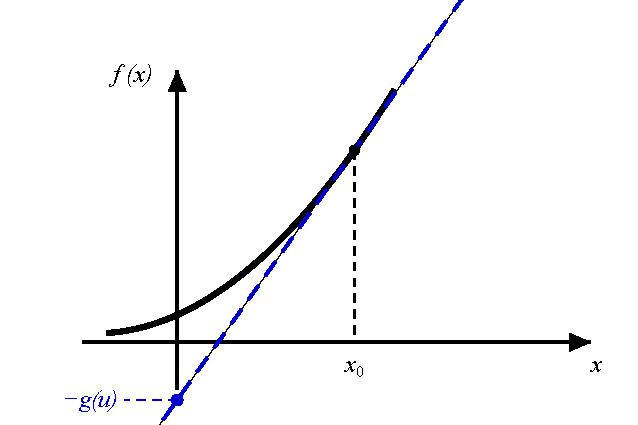
\includegraphics[width=0.58\linewidth]{Capitulo 3/Figuras/Legendre.pdf}
            \caption{Lectura geométrica de la transformada de Legendre. El valor $-g(u)$ es la ordenada en el origen de la recta tangente de pendiente $u$, de manera que describir la curva por sus tangentes contiene la misma información que describirla por sus puntos.}
            \label{fig:Legendre}
        \end{figure}

        Aplicamos la construcción al lagrangiano tomando como variable activa la velocidad generalizada y como pendiente el momento canónico \eqref{eq:MomentoCanonico}. La función transformada es la \textit{función hamiltoniana}
        \begin{equation}\label{eq:Hamiltoniano}
            H(q,p,t) \equiv \sum_{j=1}^{n}p_{j}\dot{q}_{j} - L(q,\dot{q},t),
        \end{equation}
        en la cual se entiende que todas las velocidades han sido eliminadas en favor de los momentos invirtiendo las relaciones $p_{j} = \partial L/\partial\dot{q}_{j}$. Esa inversión es posible siempre que el determinante hessiano $\det\left(\partial^{2}L/\partial\dot{q}_{j}\partial\dot{q}_{l}\right)$ no se anule, condición que se cumple para todos los lagrangianos de la forma \eqref{eq:THomogenea} porque la matriz $a_{jl}$ es definida positiva. Comparando \eqref{eq:Hamiltoniano} con \eqref{eq:hEsEnergia} vemos que el hamiltoniano es la función de energía de Jacobi expresada en las nuevas variables, y que en las condiciones allí discutidas coincide numéricamente con la energía total del sistema.

        Vamos a deducir ahora las ecuaciones de movimiento en las nuevas variables con el método de los diferenciales, que es el que hace transparente el mecanismo. Tomando el diferencial total del miembro derecho de \eqref{eq:Hamiltoniano}, tratando a $L$ como función de $(q,\dot{q},t)$,
        \begin{equation}\label{eq:DiferencialH1}
            dH = \sum_{j=1}^{n}\left(\dot{q}_{j}\,dp_{j} + p_{j}\,d\dot{q}_{j}\right)
            - \sum_{j=1}^{n}\left(\frac{\partial L}{\partial q_{j}}dq_{j} + \frac{\partial L}{\partial\dot{q}_{j}}d\dot{q}_{j}\right) - \frac{\partial L}{\partial t}dt .
        \end{equation}
        El término que contiene $d\dot{q}_{j}$ aparece dos veces con signos opuestos y coeficientes iguales, pues $\partial L/\partial\dot{q}_{j} = p_{j}$ por la definición \eqref{eq:MomentoCanonico}, de modo que
        \begin{equation}\label{eq:DiferencialH2}
            dH = \sum_{j=1}^{n}\dot{q}_{j}\,dp_{j} + \textcolor{red}{\sum_{j=1}^{n}p_{j}\,d\dot{q}_{j}} - \sum_{j=1}^{n}\frac{\partial L}{\partial q_{j}}dq_{j} - \textcolor{red}{\sum_{j=1}^{n}p_{j}\,d\dot{q}_{j}} - \frac{\partial L}{\partial t}dt,
        \end{equation}
        y los dos términos en rojo se cancelan idénticamente. Esa cancelación es el contenido entero de la transformada de Legendre: el diferencial de $H$ no contiene $d\dot{q}$, lo que demuestra que $H$ es genuinamente una función de $q$, $p$ y $t$ y no una función disfrazada de las velocidades. Queda entonces
        \begin{equation}\label{eq:DiferencialH3}
            dH = \sum_{j=1}^{n}\dot{q}_{j}\,dp_{j} - \sum_{j=1}^{n}\frac{\partial L}{\partial q_{j}}dq_{j} - \frac{\partial L}{\partial t}dt .
        \end{equation}

        Por otra parte, el diferencial de cualquier función de $(q,p,t)$ se escribe por definición como
        \begin{equation}\label{eq:DiferencialH4}
            dH = \sum_{j=1}^{n}\frac{\partial H}{\partial q_{j}}dq_{j} + \sum_{j=1}^{n}\frac{\partial H}{\partial p_{j}}dp_{j} + \frac{\partial H}{\partial t}dt .
        \end{equation}
        Como los diferenciales $dq_{j}$, $dp_{j}$ y $dt$ son independientes, la comparación término a término de \eqref{eq:DiferencialH3} y \eqref{eq:DiferencialH4} obliga a que sus coeficientes coincidan,
        \begin{equation}\label{eq:ComparacionCoef}
            \frac{\partial H}{\partial p_{j}} = \dot{q}_{j},
            \qquad
            \frac{\partial H}{\partial q_{j}} = -\frac{\partial L}{\partial q_{j}},
            \qquad
            \frac{\partial H}{\partial t} = -\frac{\partial L}{\partial t} .
        \end{equation}
        La segunda de estas relaciones se convierte en una ecuación de movimiento al invocar la ecuación de Lagrange en la forma \eqref{eq:LagrangeMomento}, que afirma $\partial L/\partial q_{j} = \dot{p}_{j}$. Reuniendo los resultados obtenemos las \textit{ecuaciones canónicas de Hamilton},
        \begin{equation}\label{eq:Hamilton}
            \boxed{\;\dot{q}_{j} = \frac{\partial H}{\partial p_{j}},
            \qquad
            \dot{p}_{j} = -\frac{\partial H}{\partial q_{j}},
            \qquad j = 1,\ldots,n .\;}
        \end{equation}

        El sistema \eqref{eq:Hamilton} consta de $2n$ ecuaciones de primer orden en lugar de $n$ de segundo orden, con lo cual el número total de constantes de integración no ha cambiado y tampoco la información física contenida. Lo que sí ha cambiado es la simetría de la descripción. En el formalismo lagrangiano las coordenadas son las protagonistas y las velocidades son cantidades derivadas de ellas; en el hamiltoniano, coordenadas y momentos aparecen en pie de igualdad, distinguidos únicamente por un signo, y esa simetría casi perfecta abre la posibilidad de transformaciones que mezclen unas con otras, cosa impensable en el lenguaje anterior. Para una partícula en un potencial, con $H = p^{2}/2m + V(x)$, las ecuaciones \eqref{eq:Hamilton} dan $\dot{x} = p/m$ y $\dot{p} = -dV/dx$, que son la definición del momento y la segunda ley de Newton escritas por separado en lugar de combinadas en una sola ecuación de segundo orden.

        Derivando $H$ respecto del tiempo a lo largo de una trayectoria y usando las propias ecuaciones canónicas, se tiene
        \begin{equation}\label{eq:ConservacionH}
            \frac{dH}{dt} = \sum_{j=1}^{n}\left(\frac{\partial H}{\partial q_{j}}\dot{q}_{j} + \frac{\partial H}{\partial p_{j}}\dot{p}_{j}\right) + \frac{\partial H}{\partial t}
            = \sum_{j=1}^{n}\left(\textcolor{red}{\frac{\partial H}{\partial q_{j}}\frac{\partial H}{\partial p_{j}}} - \textcolor{red}{\frac{\partial H}{\partial p_{j}}\frac{\partial H}{\partial q_{j}}}\right) + \frac{\partial H}{\partial t} = \frac{\partial H}{\partial t},
        \end{equation}
        donde los términos en rojo se cancelan dos a dos, recuperamos el resultado de la sección anterior en una línea: el hamiltoniano se conserva si y solo si no depende explícitamente del tiempo.

        Las $2n$ variables $(q_{1},\ldots,q_{n},p_{1},\ldots,p_{n})$ definen los puntos de una variedad de dimensión $2n$ llamada \textit{espacio de fase}, y las ecuaciones \eqref{eq:Hamilton} determinan en ella un campo vectorial cuyas curvas integrales son las trayectorias del sistema. La virtud de esta imagen es que por cada punto pasa una y solo una trayectoria, cosa que no ocurre en el espacio de configuración, donde dos movimientos distintos pueden pasar por la misma posición con velocidades diferentes; el estado dinámico queda así completamente especificado por un punto, y la evolución es un flujo.

        Ese flujo tiene una propiedad importante. Consideremos una región del espacio de fase de volumen
        \begin{equation}\label{eq:VolumenFase}
            \Omega = \int d^{n}q\,d^{n}p,
        \end{equation}
        y dejémosla evolucionar. El campo vectorial que gobierna el flujo tiene componentes $(\dot{q}_{j},\dot{p}_{j})$, y su divergencia en el espacio de fase vale
        \begin{equation}\label{eq:DivergenciaFlujo}
            \sum_{j=1}^{n}\left(\frac{\partial\dot{q}_{j}}{\partial q_{j}} + \frac{\partial\dot{p}_{j}}{\partial p_{j}}\right)
            = \sum_{j=1}^{n}\left(\frac{\partial}{\partial q_{j}}\frac{\partial H}{\partial p_{j}} - \frac{\partial}{\partial p_{j}}\frac{\partial H}{\partial q_{j}}\right)
            = \sum_{j=1}^{n}\left(\textcolor{red}{\frac{\partial^{2}H}{\partial q_{j}\partial p_{j}}} - \textcolor{red}{\frac{\partial^{2}H}{\partial p_{j}\partial q_{j}}}\right) = 0,
        \end{equation}
        donde la cancelación se debe a la igualdad de las derivadas parciales cruzadas. Un flujo de divergencia nula es incompresible, de modo que el volumen de cualquier región del espacio de fase se conserva durante la evolución, resultado conocido como \textit{teorema de Liouville} \citep{liouville1838note}. La región puede deformarse arbitrariamente, estirarse en una dirección y comprimirse en otra hasta volverse irreconocible, pero su volumen permanece constante. Este es el fundamento de la mecánica estadística clásica, y su contrapartida cuántica es la unitariedad de la evolución temporal.

    \subsection{Los corchetes de Poisson}

        La estructura algebraica del espacio de fase se expresa de manera compacta mediante la operación que Poisson introdujo en 1809 \citep{poisson1809memoire}.

        \begin{myDef}\label{def:CorchetePoisson}
            Dadas dos funciones $f(q,p,t)$ y $g(q,p,t)$ definidas sobre el espacio de fase, su \textit{corchete de Poisson} es
            \begin{equation}\label{eq:CorchetePoisson}
                \{f,g\} \equiv \sum_{j=1}^{n}\left(\frac{\partial f}{\partial q_{j}}\frac{\partial g}{\partial p_{j}} - \frac{\partial f}{\partial p_{j}}\frac{\partial g}{\partial q_{j}}\right).
            \end{equation}
        \end{myDef}

        La utilidad de esta definición se aprecia al calcular la evolución temporal de una cantidad arbitraria. Derivando $f$ a lo largo de una trayectoria y sustituyendo las ecuaciones canónicas \eqref{eq:Hamilton},
        \begin{equation}\label{eq:EvolucionPoisson}
            \frac{df}{dt} = \sum_{j=1}^{n}\left(\frac{\partial f}{\partial q_{j}}\dot{q}_{j} + \frac{\partial f}{\partial p_{j}}\dot{p}_{j}\right) + \frac{\partial f}{\partial t}
            = \sum_{j=1}^{n}\left(\frac{\partial f}{\partial q_{j}}\frac{\partial H}{\partial p_{j}} - \frac{\partial f}{\partial p_{j}}\frac{\partial H}{\partial q_{j}}\right) + \frac{\partial f}{\partial t},
        \end{equation}
        y reconociendo en el sumatorio la definición \eqref{eq:CorchetePoisson} obtenemos la \textit{ecuación de movimiento en forma de Poisson},
        \begin{equation}\label{eq:MovimientoPoisson}
            \boxed{\;\frac{df}{dt} = \{f,H\} + \frac{\partial f}{\partial t}\;}
        \end{equation}
        Toda la dinámica queda así concentrada en una sola expresión: una cantidad que no dependa explícitamente del tiempo se conserva si y solo si su corchete con el hamiltoniano se anula, y las propias ecuaciones canónicas son el caso particular $f = q_{j}$ y $f = p_{j}$, como se comprueba sustituyendo en \eqref{eq:MovimientoPoisson}.

        Las relaciones fundamentales entre las variables canónicas se obtienen directamente de la definición. Tomando $f = q_{j}$ y $g = p_{l}$, las únicas derivadas no nulas son $\partial q_{j}/\partial q_{m} = \delta_{jm}$ y $\partial p_{l}/\partial p_{m} = \delta_{lm}$, de manera que
        \begin{equation}\label{eq:CorchetesFundamentales}
            \{q_{j},p_{l}\} = \sum_{m=1}^{n}\left(\delta_{jm}\delta_{lm} - \textcolor{red}{0}\right) = \delta_{jl},
            \qquad
            \{q_{j},q_{l}\} = \{p_{j},p_{l}\} = 0 .
        \end{equation}
        El corchete de Poisson es bilineal, antisimétrico, satisface la regla de Leibniz $\{fg,h\} = f\{g,h\} + \{f,h\}g$ y cumple la identidad de Jacobi
        \begin{equation}\label{eq:IdentidadJacobi}
            \{f,\{g,h\}\} + \{g,\{h,f\}\} + \{h,\{f,g\}\} = 0,
        \end{equation}
        de modo que dota al conjunto de funciones sobre el espacio de fase de una estructura de álgebra de Lie.

        Hay una razón de fondo para habernos detenido en estas propiedades algebraicas, y es que esta es la estructura que sobrevive al paso a la mecánica cuántica. Dirac observó en 1925 que si se postula la correspondencia
        \begin{equation}\label{eq:CorrespondenciaDirac}
            \{f,g\} \;\longrightarrow\; \frac{1}{i\hbar}\left[\hat{f},\hat{g}\right],
        \end{equation}
        entonces las relaciones fundamentales \eqref{eq:CorchetesFundamentales} se convierten en las relaciones de conmutación canónicas $[\hat{q}_{j},\hat{p}_{l}] = i\hbar\delta_{jl}$, y la ecuación de movimiento \eqref{eq:MovimientoPoisson} se convierte en la ecuación de Heisenberg. En el capítulo siguiente aplicaremos exactamente este procedimiento a las amplitudes de los modos normales del campo electromagnético, y el hecho de que el álgebra resultante sea la del oscilador armónico es lo que permite hablar de fotones.

\section{Transformaciones canónicas y funciones generatrices}

    La simetría entre coordenadas y momentos en \eqref{eq:Hamilton} sugiere considerar transformaciones que mezclen unas con otras,
    \begin{equation}\label{eq:TransfCanonica}
        Q_{j} = Q_{j}(q,p,t), \qquad P_{j} = P_{j}(q,p,t),
    \end{equation}
    y preguntarse cuáles de ellas preservan la forma de las ecuaciones de movimiento. Llamaremos \textit{canónica} a una transformación tal que existe una nueva función $K(Q,P,t)$ para la cual
    \begin{equation}\label{eq:HamiltonNuevas}
        \dot{Q}_{j} = \frac{\partial K}{\partial P_{j}}, \qquad \dot{P}_{j} = -\frac{\partial K}{\partial Q_{j}} .
    \end{equation}
    El interés de estas transformaciones es puramente estratégico y es el siguiente: si consiguiéramos escoger unas variables en las cuales todas las coordenadas nuevas fuesen cíclicas, entonces todos los momentos nuevos serían constantes y el problema quedaría resuelto sin integrar nada. Llevada al extremo, esta idea conduce a la ecuación de Hamilton-Jacobi.

    La condición para que \eqref{eq:TransfCanonica} sea canónica se obtiene exigiendo que ambos juegos de variables satisfagan el principio de Hamilton. Como vimos en \eqref{eq:GaugeLagrangiano}, dos lagrangianos que difieran en una derivada total producen las mismas ecuaciones, de manera que basta con exigir
    \begin{equation}\label{eq:CondicionCanonica}
        \sum_{j=1}^{n}p_{j}\dot{q}_{j} - H = \sum_{j=1}^{n}P_{j}\dot{Q}_{j} - K + \frac{dF}{dt},
    \end{equation}
    donde $F$ es una función arbitraria llamada \textit{función generatriz}. Multiplicando por $dt$,
    \begin{equation}\label{eq:CondicionCanonicaDif}
        dF = \sum_{j=1}^{n}p_{j}\,dq_{j} - \sum_{j=1}^{n}P_{j}\,dQ_{j} + \left(K - H\right)dt .
    \end{equation}

    Si escogemos $F = F_{1}(q,Q,t)$, función de las coordenadas viejas y nuevas, su diferencial total es
    \begin{equation}\label{eq:DiferencialF1}
        dF_{1} = \sum_{j=1}^{n}\frac{\partial F_{1}}{\partial q_{j}}dq_{j} + \sum_{j=1}^{n}\frac{\partial F_{1}}{\partial Q_{j}}dQ_{j} + \frac{\partial F_{1}}{\partial t}dt,
    \end{equation}
    y comparando coeficientes con \eqref{eq:CondicionCanonicaDif}, lo que es lícito porque $dq_{j}$, $dQ_{j}$ y $dt$ son independientes, resultan las relaciones de transformación
    \begin{equation}\label{eq:RelacionesF1}
        p_{j} = \frac{\partial F_{1}}{\partial q_{j}},
        \qquad
        P_{j} = -\frac{\partial F_{1}}{\partial Q_{j}},
        \qquad
        K = H + \frac{\partial F_{1}}{\partial t} .
    \end{equation}
    La función generatriz determina así por completo la transformación: dadas $F_{1}$ y las primeras $n$ relaciones, se despejan las $Q_{j}$ en términos de $(q,p,t)$, y las segundas dan entonces los momentos nuevos.

    Las demás variantes se obtienen aplicando transformadas de Legendre a $F_{1}$ para cambiar el par de variables independientes. La que nos interesará es la de tipo dos, definida por
    \begin{equation}\label{eq:F2}
        F_{2}(q,P,t) = F_{1}(q,Q,t) + \sum_{j=1}^{n}Q_{j}P_{j},
    \end{equation}
    cuyo diferencial, usando \eqref{eq:RelacionesF1}, vale
    \begin{equation}\label{eq:DiferencialF2}
        dF_{2} = \sum_{j=1}^{n}p_{j}\,dq_{j} - \textcolor{red}{\sum_{j=1}^{n}P_{j}\,dQ_{j}} + \textcolor{red}{\sum_{j=1}^{n}P_{j}\,dQ_{j}} + \sum_{j=1}^{n}Q_{j}\,dP_{j} + \left(K-H\right)dt,
    \end{equation}
    donde los términos en rojo se cancelan, de modo que las relaciones de transformación son
    \begin{equation}\label{eq:RelacionesF2}
        p_{j} = \frac{\partial F_{2}}{\partial q_{j}},
        \qquad
        Q_{j} = \frac{\partial F_{2}}{\partial P_{j}},
        \qquad
        K = H + \frac{\partial F_{2}}{\partial t} .
    \end{equation}
    Obsérvese que $F_{2} = \sum_{j}q_{j}P_{j}$ genera la transformación identidad, lo que confirma que este tipo es el adecuado para describir transformaciones próximas a no hacer nada.

\section{La ecuación de Hamilton-Jacobi}

        Vamos a llevar ahora la estrategia al extremo, pidiendo que la transformación canónica sea tan eficaz que el nuevo hamiltoniano se anule idénticamente,
        \begin{equation}\label{eq:KCero}
            K = 0 .
        \end{equation}
        Si tal transformación existe, las ecuaciones de movimiento en las variables nuevas \eqref{eq:HamiltonNuevas} se reducen a $\dot{Q}_{j} = 0$ y $\dot{P}_{j} = 0$, de manera que las $2n$ variables nuevas son todas constantes del movimiento y el problema dinámico queda completamente resuelto: basta invertir la transformación para obtener $q_{j}(t)$.

        Usando una generatriz de tipo dos y denotándola tradicionalmente por $S$, la tercera de las relaciones \eqref{eq:RelacionesF2} junto con la exigencia \eqref{eq:KCero} da
        \begin{equation}\label{eq:HJPrevia}
            H\left(q,p,t\right) + \frac{\partial S}{\partial t} = 0,
        \end{equation}
        y sustituyendo en ella los momentos por sus expresiones $p_{j} = \partial S/\partial q_{j}$, que es la primera de las relaciones \eqref{eq:RelacionesF2}, obtenemos la \textit{ecuación de Hamilton-Jacobi},
        \begin{equation}\label{eq:HamiltonJacobi}
            \boxed{\;H\left(q_{1},\ldots,q_{n},\frac{\partial S}{\partial q_{1}},\ldots,\frac{\partial S}{\partial q_{n}},t\right) + \frac{\partial S}{\partial t} = 0 .\;}
        \end{equation}

        Se trata de una única ecuación en derivadas parciales de primer orden para la función $S(q,t)$, llamada \textit{función principal de Hamilton}. Hemos cambiado $2n$ ecuaciones diferenciales ordinarias por una sola ecuación en derivadas parciales, lo cual a primera vista parece un retroceso, y en muchos problemas concretos efectivamente lo es; pero el cambio tiene dos virtudes que lo compensan con creces. La primera es práctica: cuando la ecuación admite separación de variables, la solución se reduce a $n$ cuadraturas independientes y el problema se resuelve sin integrar ninguna ecuación diferencial acoplada. La segunda es conceptual, y es la que nos interesa aquí: la ecuación de Hamilton-Jacobi es la formulación de la mecánica clásica que más se parece a una teoría ondulatoria, porque describe la evolución de una función escalar definida sobre todo el espacio de configuración en lugar de la evolución de una trayectoria. Esa semejanza no es casual y es la que Schrödinger explotará.

        Para un sistema conservativo, en el cual $H$ no depende explícitamente del tiempo, la dependencia temporal de $S$ puede separarse escribiendo
        \begin{equation}\label{eq:SeparacionTemporal}
            S(q,t) = W(q) - Et,
        \end{equation}
        pues sustituyendo en \eqref{eq:HamiltonJacobi} se obtiene $H(q,\partial W/\partial q) = E$, ecuación que ya no contiene el tiempo y en la cual $E$ es la constante de separación, identificable con la energía. La función $W$ se llama \textit{función característica de Hamilton}.

        La función $S$ no es un artificio de cálculo: es la acción, y lo demostramos porque de ello depende toda la interpretación posterior. La derivada temporal total de $S$ a lo largo de una trayectoria efectiva del sistema vale
        \begin{equation}\label{eq:DerivadaS}
            \frac{dS}{dt} = \sum_{j=1}^{n}\frac{\partial S}{\partial q_{j}}\dot{q}_{j} + \frac{\partial S}{\partial t},
        \end{equation}
        y sustituyamos las dos identificaciones que la propia construcción nos ha dado, a saber $\partial S/\partial q_{j} = p_{j}$ y, por \eqref{eq:HJPrevia}, $\partial S/\partial t = -H$,
        \begin{equation}\label{eq:DerivadaS2}
            \frac{dS}{dt} = \sum_{j=1}^{n}p_{j}\dot{q}_{j} - H = L,
        \end{equation}
        donde el último paso es la definición \eqref{eq:Hamiltoniano} del hamiltoniano despejada para $L$. Integrando entre dos instantes,
        \begin{equation}\label{eq:SEsAccion}
            S = \int L\,dt + \text{constante},
        \end{equation}
        de manera que la función principal de Hamilton es la acción evaluada sobre la trayectoria efectiva del sistema, considerada como función del punto final y del instante final. Esta es una diferencia sutil pero decisiva respecto de la acción \eqref{eq:Accion} de la sección anterior: allí $S$ era un funcional definido sobre todos los caminos imaginables con extremos fijos, mientras que aquí es una función ordinaria de las coordenadas finales, obtenida al evaluar la acción únicamente sobre el camino clásico que llega a ese punto.

        \begin{figure}[htbp]
            \centering
            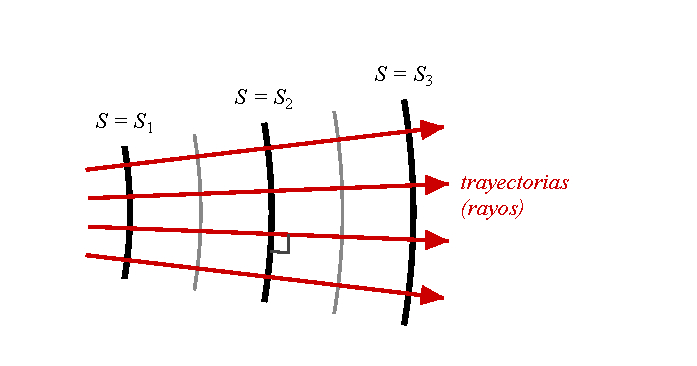
\includegraphics[width=0.62\linewidth]{Capitulo 3/Figuras/FrentesAccion.pdf}
            \caption{Superficies de acción constante y trayectorias mecánicas. El momento es el gradiente de $S$, de modo que las trayectorias cortan perpendicularmente a los frentes, exactamente como los rayos luminosos cortan a los frentes de onda.}
            \label{fig:FrentesAccion}
        \end{figure}

        La relación $p_{j} = \partial S/\partial q_{j}$ admite entonces una lectura geométrica que es el corazón de la analogía óptico-mecánica. Las superficies $S(q,t) = \text{constante}$ forman una familia que barre el espacio de configuración a medida que transcurre el tiempo, y el gradiente de $S$, que es perpendicular a esas superficies, es el momento de la partícula. \textbf{Las trayectorias mecánicas son, por tanto, las curvas ortogonales a las superficies de acción constante}, exactamente como los rayos luminosos son las curvas ortogonales a los frentes de onda. La sección siguiente hace explícita esa correspondencia.

        Ilustremos el método en el caso más simple posible, donde todo puede calcularse hasta el final. Para una partícula libre en una dimensión el hamiltoniano es $H = p^{2}/2m$, y la ecuación \eqref{eq:HamiltonJacobi} se escribe
        \begin{equation}\label{eq:HJLibre}
            \frac{1}{2m}\left(\frac{\partial S}{\partial x}\right)^{2} + \frac{\partial S}{\partial t} = 0 .
        \end{equation}
        Separando la dependencia temporal según \eqref{eq:SeparacionTemporal} con $S = W(x) - Et$, y sustituyendo,
        \begin{equation}\label{eq:HJLibre2}
            \frac{1}{2m}\left(\frac{dW}{dx}\right)^{2} = E
            \qquad\Longrightarrow\qquad
            \frac{dW}{dx} = \sqrt{2mE},
        \end{equation}
        que se integra de inmediato dando $W = \sqrt{2mE}\,x$, de modo que
        \begin{equation}\label{eq:SLibre}
            S(x,t) = \sqrt{2mE}\,x - Et .
        \end{equation}
        Las superficies de acción constante son en este caso planos perpendiculares al eje, y avanzan con velocidad
        \begin{equation}\label{eq:VelocidadFrente}
            u = \frac{E}{\sqrt{2mE}} = \sqrt{\frac{E}{2m}} = \frac{v}{2},
        \end{equation}
        donde $v = \sqrt{2E/m}$ es la velocidad de la partícula. El resultado es contraintuitivo: los frentes de acción constante se mueven a la mitad de la velocidad de la partícula, de manera que la analogía con una onda, si ha de mantenerse, exige que la partícula corresponda no a la velocidad de fase de esa onda sino a algo distinto. Volveremos sobre esta discrepancia al discutir la velocidad de grupo, porque es exactamente el punto en el que de Broglie y Schrödinger tuvieron que ser cuidadosos.

        Para completar el ejemplo, la constante de integración $E$ hace el papel del momento nuevo $P$, y la coordenada nueva conjugada se obtiene de la segunda relación \eqref{eq:RelacionesF2},
        \begin{equation}\label{eq:QLibre}
            Q = \frac{\partial S}{\partial E} = \sqrt{\frac{m}{2E}}\,x - t = \text{constante},
        \end{equation}
        de donde, despejando, $x = \sqrt{2E/m}\,(t + Q) = v\,t + x_{0}$, que es el movimiento rectilíneo uniforme esperado. El método ha producido la solución sin integrar ninguna ecuación de movimiento.

    \subsection{Ejemplo: el oscilador armónico y su acción clásica}

        El segundo ejemplo es el que necesitaremos literalmente más adelante, porque el campo electromagnético cuantizado es una colección de osciladores armónicos y la propagación de los fotones se describirá mediante el propagador de un oscilador. Calcularemos aquí la acción clásica del oscilador como función de sus extremos, que es el ingrediente central de ese propagador.

        El lagrangiano y el hamiltoniano de un oscilador de masa $m$ y frecuencia $\omega$ son
        \begin{equation}\label{eq:LagrangianoOsc}
            L = \frac{1}{2}m\dot{q}^{2} - \frac{1}{2}m\omega^{2}q^{2},
            \qquad
            H = \frac{p^{2}}{2m} + \frac{1}{2}m\omega^{2}q^{2},
        \end{equation}
        y la ecuación de movimiento que se sigue de \eqref{eq:EulerLagrange2} es $\ddot{q} + \omega^{2}q = 0$, cuya solución general escribimos en la forma
        \begin{equation}\label{eq:SolucionOsc}
            q(s) = A\cos\omega s + B\sin\omega s .
        \end{equation}
        Impongamos las condiciones de contorno propias de un problema variacional, es decir, valores prescritos en los dos extremos del intervalo temporal, $q(0) = q_{I}$ y $q(t) = q_{F}$. La primera da inmediatamente $A = q_{I}$, y la segunda
        \begin{equation}\label{eq:CondicionB}
            q_{F} = q_{I}\cos\omega t + B\sin\omega t
            \qquad\Longrightarrow\qquad
            B = \frac{q_{F} - q_{I}\cos\omega t}{\sin\omega t},
        \end{equation}
        expresión que exige $\sin\omega t \neq 0$, condición cuyo significado físico discutiremos al final. La trayectoria clásica que une ambos puntos es por tanto
        \begin{equation}\label{eq:TrayectoriaOsc}
            q_{\mathrm{cl}}(s) = q_{I}\cos\omega s + \frac{q_{F} - q_{I}\cos\omega t}{\sin\omega t}\,\sin\omega s .
        \end{equation}

        Para evaluar la acción sobre esta trayectoria simplificamos primero el integrando mediante una integración por partes, lo que evita tener que elevar al cuadrado la expresión anterior. Partimos de
        \begin{equation}\label{eq:AccionOsc1}
            S_{\mathrm{cl}} = \int_{0}^{t}\left(\frac{1}{2}m\dot{q}^{2} - \frac{1}{2}m\omega^{2}q^{2}\right)ds,
        \end{equation}
        y transformamos el término cinético escribiendo $\dot{q}^{2} = \frac{d}{ds}(q\dot{q}) - q\ddot{q}$, identidad que no es más que la regla del producto reordenada,
        \begin{equation}\label{eq:AccionOsc2}
            S_{\mathrm{cl}} = \frac{m}{2}\left[q\dot{q}\right]_{0}^{t} - \frac{m}{2}\int_{0}^{t} q\left(\ddot{q} + \textcolor{blue}{\omega^{2}q}\right)ds,
        \end{equation}
        donde el término en azul se ha agrupado deliberadamente con $\ddot{q}$ para formar el miembro izquierdo de la ecuación de movimiento. Como la trayectoria es clásica, ese paréntesis se anula idénticamente y la integral desaparece por completo,
        \begin{equation}\label{eq:AccionOscFrontera}
            S_{\mathrm{cl}} = \frac{m}{2}\left[q_{\mathrm{cl}}(t)\dot{q}_{\mathrm{cl}}(t) - q_{\mathrm{cl}}(0)\dot{q}_{\mathrm{cl}}(0)\right].
        \end{equation}
        El resultado no es privativo del oscilador. La acción clásica de cualquier sistema cuadrático se reduce a un término de frontera, lo cual explica por qué el oscilador armónico y la partícula libre son los únicos sistemas cuyo propagador puede escribirse en forma cerrada elemental.

        Solo resta evaluar las velocidades en los extremos. Derivando \eqref{eq:TrayectoriaOsc},
        \begin{equation}\label{eq:VelocidadOsc}
            \dot{q}_{\mathrm{cl}}(s) = -q_{I}\omega\sin\omega s + \omega\,\frac{q_{F}-q_{I}\cos\omega t}{\sin\omega t}\cos\omega s,
        \end{equation}
        de donde, en $s=0$, donde $\sin 0 = 0$ y $\cos 0 = 1$,
        \begin{equation}\label{eq:VelocidadInicial}
            \dot{q}_{\mathrm{cl}}(0) = \omega\,\frac{q_{F}-q_{I}\cos\omega t}{\sin\omega t},
        \end{equation}
        y en $s=t$,
        \begin{equation}\label{eq:VelocidadFinal}
            \dot{q}_{\mathrm{cl}}(t) = -q_{I}\omega\sin\omega t + \omega\,\frac{\left(q_{F}-q_{I}\cos\omega t\right)\cos\omega t}{\sin\omega t}
            = \omega\,\frac{-q_{I}\sin^{2}\omega t + q_{F}\cos\omega t - q_{I}\cos^{2}\omega t}{\sin\omega t},
        \end{equation}
        donde hemos puesto todo sobre el denominador común $\sin\omega t$. Los dos términos en $q_{I}$ se combinan mediante la identidad pitagórica $\sin^{2}\omega t + \cos^{2}\omega t = 1$,
        \begin{equation}\label{eq:VelocidadFinal2}
            \dot{q}_{\mathrm{cl}}(t) = \omega\,\frac{q_{F}\cos\omega t - q_{I}}{\sin\omega t} .
        \end{equation}

        Sustituyendo \eqref{eq:VelocidadInicial} y \eqref{eq:VelocidadFinal2} en \eqref{eq:AccionOscFrontera},
        \begin{equation}\label{eq:AccionOsc3}
            S_{\mathrm{cl}} = \frac{m\omega}{2\sin\omega t}\left[q_{F}\left(q_{F}\cos\omega t - q_{I}\right) - q_{I}\left(q_{F} - q_{I}\cos\omega t\right)\right],
        \end{equation}
        y desarrollando los dos productos del corchete,
        \begin{equation}\label{eq:AccionOsc4}
            S_{\mathrm{cl}} = \frac{m\omega}{2\sin\omega t}\left[q_{F}^{2}\cos\omega t - q_{I}q_{F} - q_{I}q_{F} + q_{I}^{2}\cos\omega t\right],
        \end{equation}
        de manera que los dos términos cruzados, que son idénticos, se suman y obtenemos finalmente
        \begin{equation}\label{eq:AccionOscilador}
            \boxed{\;S_{\mathrm{cl}}(q_{F},t;q_{I},0) = \frac{m\omega}{2\sin\omega t}\left[\left(q_{I}^{2}+q_{F}^{2}\right)\cos\omega t - 2q_{I}q_{F}\right].\;}
        \end{equation}

        Merece la pena detenerse en esta expresión, porque es exactamente el exponente que aparecerá en el propagador del campo electromagnético cuantizado. Dividiendo numerador y denominador por $\sin\omega t$ el resultado puede escribirse de manera equivalente como
        \begin{equation}\label{eq:AccionOsciladorCot}
            S_{\mathrm{cl}} = \frac{m\omega}{2}\left[\left(q_{I}^{2}+q_{F}^{2}\right)\cot\omega t - \frac{2q_{I}q_{F}}{\sin\omega t}\right],
        \end{equation}
        y esta es, salvo el factor de masa, la combinación de una cotangente multiplicando a la suma de cuadrados y de una cosecante multiplicando al producto cruzado que reconoceremos en el núcleo de la transformada de Fourier fraccionaria y en la integral de difracción de Fresnel. La estructura matemática que conecta la propagación de la luz clásica con la evolución de un fotón está contenida, en germen, en esta expresión puramente mecánica.

        Vale la pena ver qué ocurre cuando $\omega t$ se aproxima a un múltiplo entero de $\pi$. El denominador $\sin\omega t$ se anula y la acción diverge, salvo para pares de puntos particulares; físicamente, tras medio período todas las trayectorias que parten de $q_{I}$ vuelven a converger en el mismo punto, de manera que el problema de contorno deja de tener solución única. Estos instantes se llaman \textit{puntos conjugados} o \textit{cáusticas}, y la divergencia de la acción en ellos es el análogo mecánico exacto del foco de un sistema óptico, donde la aproximación de rayos también deja de ser válida. En el lenguaje del capítulo dedicado a la difracción, un punto conjugado es aquel en el cual la fase estacionaria degenera y el cálculo asintótico debe refinarse.

    \subsection{La analogía óptico-mecánica de Hamilton}

        Estamos ya en condiciones de establecer con precisión la correspondencia que Hamilton descubrió en 1834 y que constituye el puente hacia la mecánica ondulatoria.

        En óptica geométrica, el principio de Fermat establece que un rayo luminoso entre dos puntos recorre un camino de longitud óptica estacionaria,
        \begin{equation}\label{eq:Fermat}
            \delta\int_{A}^{B} n(\mathbf{r})\,dl = 0,
        \end{equation}
        donde $n$ es el índice de refracción. En mecánica, el principio de Maupertuis, que se obtiene del de Hamilton restringiéndose a variaciones que conservan la energía, establece que la trayectoria de una partícula satisface
        \begin{equation}\label{eq:Maupertuis}
            \delta\int_{A}^{B} p\,dl = 0,
            \qquad
            p = \sqrt{2m\left[E - V(\mathbf{r})\right]} .
        \end{equation}
        Las dos expresiones son formalmente idénticas, y la correspondencia entre ellas exige identificar
        \begin{equation}\label{eq:DiccionarioHamilton}
            n(\mathbf{r}) \;\longleftrightarrow\; \sqrt{2m\left[E-V(\mathbf{r})\right]} = p,
        \end{equation}
        es decir, el índice de refracción del medio mecánico es el momento de la partícula. Un potencial atractivo actúa sobre las trayectorias exactamente como un medio de índice creciente actúa sobre los rayos, y la refracción de una partícula al atravesar un escalón de potencial obedece una ley de Snell con los momentos en lugar de los índices.

        La correspondencia se extiende al nivel de las funciones. En óptica, la fase de la onda define la \textit{eikonal} $\mathcal{L}(\mathbf{r})$ mediante $\mathcal{E} \sim \exp\left[ik_{0}\mathcal{L}\right]$, y los frentes de onda son sus superficies de nivel, mientras que en mecánica es la función característica $W$ la que juega ese papel. Al sustituir la forma eikonal en la ecuación de Helmholtz y quedarse con el término dominante en el límite de longitud de onda corta se obtiene la \textit{ecuación de la eikonal},
        \begin{equation}\label{eq:Eikonal}
            \left\|\nabla\mathcal{L}\right\|^{2} = n^{2}(\mathbf{r}),
        \end{equation}
        y al sustituir $p = \nabla W$ en $H = E$ se obtiene la ecuación de Hamilton-Jacobi independiente del tiempo,
        \begin{equation}\label{eq:HJIndependiente}
            \left\|\nabla W\right\|^{2} = 2m\left[E - V(\mathbf{r})\right] .
        \end{equation}
        Las dos ecuaciones tienen la misma forma, y el diccionario \eqref{eq:DiccionarioHamilton} las transforma una en otra.

        Hamilton se detuvo aquí, y la razón es comprensible: en su época no existía ningún indicio experimental de que la mecánica clásica fuese el límite de otra cosa, de manera que la analogía era una elegancia matemática sin consecuencias. La pregunta que Hamilton no hizo, y que noventa años después haría de Broglie, es la siguiente: si la mecánica clásica es a la mecánica verdadera lo que la óptica geométrica es a la óptica ondulatoria, entonces debe existir una ecuación de ondas subyacente cuya aproximación eikonal sea la ecuación de Hamilton-Jacobi, y esa ecuación describiría el comportamiento de la materia allí donde la aproximación de rayos falla. La sección siguiente reconstruye el camino que llevó de esa pregunta a la ecuación de Schrödinger.

\section{De la ecuación de Hamilton-Jacobi a la ecuación de Schrödinger}

        En su tesis doctoral de 1924 Louis de Broglie propuso que la dualidad que Einstein había establecido para la luz debía extenderse a la materia, de manera que a toda partícula de momento $p$ le corresponde una onda de longitud
        \begin{equation}\label{eq:deBroglie}
            \lambda = \frac{h}{p},
            \qquad\text{equivalentemente}\qquad
            k = \frac{2\pi}{\lambda} = \frac{p}{\hbar},
        \end{equation}
        y a toda energía $E$ una frecuencia
        \begin{equation}\label{eq:PlanckEinstein}
            \omega = \frac{E}{\hbar} .
        \end{equation}
        Estas dos relaciones bastan para cerrar el diccionario de Hamilton, porque convierten la correspondencia formal entre la eikonal y la función característica en una afirmación cuantitativa sobre una onda física.

        Comprobémoslo. Si la fase de esa onda ha de ser proporcional a la función principal de Hamilton, como exige la identificación de los frentes de onda con las superficies de acción constante, entonces escribimos
        \begin{equation}\label{eq:FaseEsAccion}
            \Phi(\mathbf{r},t) = \frac{S(\mathbf{r},t)}{\hbar} = \frac{W(\mathbf{r}) - Et}{\hbar},
        \end{equation}
        y las dos relaciones de de Broglie se siguen de inmediato: el gradiente de la fase es $\nabla\Phi = \nabla W/\hbar = \mathbf{p}/\hbar$, que es el vector de onda, y la derivada temporal es $\partial\Phi/\partial t = -E/\hbar$, que es la frecuencia angular con el signo convencional. La constante $\hbar$ entra en la teoría únicamente como el factor de conversión entre la acción y la fase, y esa es toda su función: sin ella, la exponencial de una acción no tendría sentido dimensional.

        Podemos aclarar de una vez la dificultad que mencionamos al tratar la partícula libre, porque es la que estuvo a punto de descarrilar la construcción. La velocidad con que avanzan los frentes de fase constante es
        \begin{equation}\label{eq:VelocidadFase}
            u = \frac{\omega}{k} = \frac{E/\hbar}{p/\hbar} = \frac{E}{p} = \frac{E}{\sqrt{2m\left[E-V\right]}},
        \end{equation}
        que para una partícula libre no relativista vale $u = (p^{2}/2m)/p = v/2$, es decir, la mitad de la velocidad de la partícula, tal como habíamos obtenido en \eqref{eq:VelocidadFrente}. Si la partícula fuese la onda, la contradicción sería fatal. La solución está en que una partícula localizada no corresponde a una onda monocromática sino a un paquete construido superponiendo un intervalo estrecho de frecuencias, y un paquete no viaja con la velocidad de fase sino con la \textit{velocidad de grupo},
        \begin{equation}\label{eq:VelocidadGrupo}
            v_{g} = \frac{d\omega}{dk} = \frac{d(E/\hbar)}{d(p/\hbar)} = \frac{dE}{dp} = \frac{d}{dp}\left(\frac{p^{2}}{2m}\right) = \frac{p}{m} = v,
        \end{equation}
        que sí coincide con la velocidad clásica. Obsérvese además que la velocidad de fase \eqref{eq:VelocidadFase} depende del origen desde el cual se mida la energía, pues sumar una constante al potencial cambia $E$ y por tanto cambia $u$, mientras que la velocidad de grupo \eqref{eq:VelocidadGrupo}, al ser una derivada, no se ve afectada. La velocidad de fase no es una cantidad física y la velocidad de grupo sí lo es, y esta observación, que hoy resulta rutinaria en el estudio de la coherencia y de la propagación de pulsos, fue en 1924 el argumento decisivo que permitió a de Broglie sostener su hipótesis frente a la objeción más obvia que se le podía hacer.

        Disponemos ya de todos los elementos para ejecutar el programa. La lógica es la siguiente: si la mecánica clásica es el límite de rayos de una teoría ondulatoria, escribamos la ecuación de ondas más simple posible, la ecuación de onda clásica, dotémosla de la velocidad de fase que la ecuación de Hamilton-Jacobi prescribe, e impongamos las relaciones de de Broglie. Veremos que ese procedimiento produce, sin ningún ingrediente adicional, la ecuación de Schrödinger.

        Partimos entonces de la ecuación de onda clásica para una función escalar $\Psi(\mathbf{r},t)$ que se propaga en un medio con velocidad de fase $u(\mathbf{r})$ dependiente de la posición,
        \begin{equation}\label{eq:OndaClasica}
            \nabla^{2}\Psi(\mathbf{r},t) - \frac{1}{u^{2}(\mathbf{r})}\frac{\partial^{2}\Psi(\mathbf{r},t)}{\partial t^{2}} = 0,
        \end{equation}
        que es exactamente la ecuación con la que iniciamos el estudio de la difracción escalar en \ref{Sec:Diffraction}, allí con $u = c/n$ y aquí con la velocidad de fase mecánica \eqref{eq:VelocidadFase}. La analogía óptico-mecánica no es aquí una metáfora: estamos usando literalmente la misma ecuación con otro índice de refracción.

        Busquemos soluciones monocromáticas, es decir, de frecuencia bien definida, separando la dependencia temporal en la forma
        \begin{equation}\label{eq:SeparacionMonocromatica}
            \Psi(\mathbf{r},t) = \psi(\mathbf{r})\,e^{-i\omega t} .
        \end{equation}
        Derivando dos veces respecto del tiempo, cada derivada baja un factor $-i\omega$,
        \begin{equation}\label{eq:SegundaDerivadaTemporal}
            \frac{\partial^{2}\Psi}{\partial t^{2}} = \left(-i\omega\right)^{2}\psi(\mathbf{r})e^{-i\omega t} = -\omega^{2}\,\psi(\mathbf{r})\,e^{-i\omega t},
        \end{equation}
        y sustituyendo en \eqref{eq:OndaClasica},
        \begin{equation}\label{eq:HelmholtzPaso}
            \left[\nabla^{2}\psi(\mathbf{r}) + \frac{\omega^{2}}{u^{2}(\mathbf{r})}\psi(\mathbf{r})\right]\textcolor{red}{e^{-i\omega t}} = 0 .
        \end{equation}
        La exponencial marcada en rojo nunca se anula, de modo que puede dividirse la ecuación por ella, y queda la ecuación de Helmholtz
        \begin{equation}\label{eq:HelmholtzMecanico}
            \nabla^{2}\psi + \frac{\omega^{2}}{u^{2}}\psi = 0 .
        \end{equation}
        Este es el mismo paso que dimos al deducir la ecuación de Helmholtz óptica, y hasta aquí no hemos usado ninguna hipótesis cuántica: \eqref{eq:HelmholtzMecanico} es física ondulatoria del siglo XIX.

        El ingrediente cuántico entra ahora, y entra por una sola puerta. Sustituimos en el coeficiente $\omega^{2}/u^{2}$ la frecuencia dada por la relación de Planck y Einstein \eqref{eq:PlanckEinstein} y la velocidad de fase dada por Hamilton-Jacobi \eqref{eq:VelocidadFase},
        \begin{equation}\label{eq:CoeficienteSustituido}
            \frac{\omega^{2}}{u^{2}} = \frac{\left(E/\hbar\right)^{2}}{\left(E/p\right)^{2}}
            = \frac{E^{2}}{\hbar^{2}}\cdot\frac{p^{2}}{E^{2}}
            = \frac{p^{2}}{\hbar^{2}},
        \end{equation}
        donde el cuadrado de la energía se cancela por completo entre el numerador y el denominador. Este detalle es importante: la energía total desaparece del coeficiente y solo sobrevive el momento, que es precisamente la cantidad que la relación de de Broglie \eqref{eq:deBroglie} conecta con la longitud de onda, de modo que el coeficiente de \eqref{eq:HelmholtzMecanico} es simplemente $k^{2} = (2\pi/\lambda)^{2}$, tal y como ocurre en la óptica.

        Sustituyendo ahora el momento mecánico $p^{2} = 2m\left[E - V(\mathbf{r})\right]$, que es la relación que define la velocidad de fase en \eqref{eq:VelocidadFase} y que proviene de la ecuación de Hamilton-Jacobi independiente del tiempo \eqref{eq:HJIndependiente},
        \begin{equation}\label{eq:SchrodingerPaso1}
            \nabla^{2}\psi + \frac{2m}{\hbar^{2}}\left[E - V(\mathbf{r})\right]\psi = 0 .
        \end{equation}
        Multiplicando por $-\hbar^{2}/2m$ y reordenando los términos de manera que la energía quede aislada a la derecha,
        \begin{equation}\label{eq:SchrodingerEstacionaria}
            \boxed{\;-\frac{\hbar^{2}}{2m}\nabla^{2}\psi(\mathbf{r}) + V(\mathbf{r})\,\psi(\mathbf{r}) = E\,\psi(\mathbf{r}),\;}
        \end{equation}
        que es la \textit{ecuación de Schrödinger independiente del tiempo}, tal como apareció en la primera comunicación de enero de 1926 \citep{schrodinger1926quantisierung}.

        Vale la pena mirar lo ocurrido. No hemos postulado nada que no estuviera ya en la mesa: la ecuación de onda clásica es del siglo XVIII, la velocidad de fase la fija la ecuación de Hamilton-Jacobi del siglo XIX, y las dos únicas relaciones nuevas son $E = \hbar\omega$ y $p = \hbar k$. El contenido físico de \eqref{eq:SchrodingerEstacionaria} tampoco está en su forma, que es la de una ecuación de Helmholtz con índice de refracción variable, sino en las condiciones de contorno: exigir que $\psi$ sea finita, univaluada y de cuadrado integrable en todo el espacio selecciona únicamente ciertos valores de $E$, exactamente igual que exigir que una cuerda esté sujeta en sus dos extremos selecciona únicamente ciertas frecuencias de vibración. La cuantización de la energía deja de ser un postulado ad hoc, como lo era en el modelo de Bohr, y se convierte en un problema de valores propios de una ecuación diferencial, que es precisamente lo que anuncia el título de la memoria de Schrödinger, \textit{Quantisierung als Eigenwertproblem}, la cuantización como problema de valores propios.

    \subsection{El camino que siguió Schrödinger: la sustitución exponencial}

        La reconstrucción anterior es la que se presenta habitualmente y es la que Schrödinger desarrolló con detalle en su segunda comunicación \citep{schrodinger1926quantisierungII}, pero no es la que aparece en la primera. El razonamiento original es más breve y más audaz, y merece reproducirse porque en él la ecuación de Hamilton-Jacobi no es un ingrediente auxiliar sino el punto de partida literal.

        Schrödinger parte de la ecuación de Hamilton-Jacobi independiente del tiempo para un sistema conservativo, que escribimos en la forma
        \begin{equation}\label{eq:HJPartida}
            \frac{1}{2m}\left\|\nabla W\right\|^{2} + V(\mathbf{r}) = E,
        \end{equation}
        e introduce una nueva función incógnita $\psi$ mediante la sustitución
        \begin{equation}\label{eq:SustitucionLog}
            W = K\ln\psi,
        \end{equation}
        donde $K$ es por el momento una constante con dimensiones de acción, cuyo valor se fijará al final. La motivación de esta sustitución es que convierte la relación multiplicativa entre las funciones de onda de subsistemas independientes en la relación aditiva que la acción satisface, pues la acción de dos sistemas independientes se suma mientras que sus amplitudes se multiplican, y el logaritmo es la única función que convierte productos en sumas.

        El gradiente de \eqref{eq:SustitucionLog} se obtiene con la regla de la cadena,
        \begin{equation}\label{eq:GradienteLog}
            \nabla W = K\,\frac{\nabla\psi}{\psi},
        \end{equation}
        y sustituyámoslo en \eqref{eq:HJPartida},
        \begin{equation}\label{eq:HJSustituida}
            \frac{K^{2}}{2m}\frac{\left\|\nabla\psi\right\|^{2}}{\psi^{2}} + V = E .
        \end{equation}
        Multiplicando por $2m\psi^{2}$ y pasando todo a un miembro obtenemos una expresión polinómica, libre ya de denominadores,
        \begin{equation}\label{eq:HJPolinomica}
            K^{2}\left\|\nabla\psi\right\|^{2} - 2m\left[E - V\right]\psi^{2} = 0 .
        \end{equation}

        Aquí se produce el paso decisivo, y también el más discutido. Schrödinger no intenta resolver \eqref{eq:HJPolinomica}, que sigue siendo una ecuación de Hamilton-Jacobi disfrazada y por tanto sigue describiendo mecánica clásica. Lo que hace es sustituir la exigencia de que la expresión se anule punto a punto por la exigencia, mucho más débil, de que su integral sobre todo el espacio sea estacionaria,
        \begin{equation}\label{eq:FuncionalSchrodinger}
            \delta J[\psi] = 0,
            \qquad
            J[\psi] = \int_{\mathbb{R}^{3}}\left\{K^{2}\left\|\nabla\psi\right\|^{2} - 2m\left[E - V(\mathbf{r})\right]\psi^{2}\right\}d^{3}r .
        \end{equation}
        La justificación que Schrödinger ofrece es de analogía: así como el principio de Fermat, que exige la estacionariedad de una integral, da la óptica geométrica correcta pero solo describe rayos, y la descripción completa exige una ecuación de ondas, del mismo modo la mecánica de trayectorias debe ceder el paso a un principio variacional sobre un campo definido en todo el espacio. Es un salto, y él mismo lo reconoce; su validación es que funciona.

        La variación indicada en \eqref{eq:FuncionalSchrodinger} es un ejercicio del cálculo de variaciones idéntico al de la sección anterior salvo que ahora la variable independiente es el punto del espacio y no el tiempo. Variando $\psi\rightarrow\psi + \delta\psi$ y quedándonos con el primer orden,
        \begin{equation}\label{eq:VariacionJ}
            \delta J = \int_{\mathbb{R}^{3}}\left\{2K^{2}\,\nabla\psi\cdot\nabla\delta\psi - 4m\left[E-V\right]\psi\,\delta\psi\right\}d^{3}r,
        \end{equation}
        donde el factor dos del primer término proviene de derivar un cuadrado y el factor cuatro del segundo de derivar el otro cuadrado multiplicado por el dos que ya estaba. Para poder factorizar $\delta\psi$ hay que quitarle el gradiente al primer término, y eso se consigue con la identidad vectorial
        \begin{equation}\label{eq:IdentidadDivergencia}
            \nabla\cdot\left(\delta\psi\,\nabla\psi\right) = \nabla\delta\psi\cdot\nabla\psi + \delta\psi\,\nabla^{2}\psi
            \qquad\Longrightarrow\qquad
            \nabla\psi\cdot\nabla\delta\psi = \nabla\cdot\left(\delta\psi\,\nabla\psi\right) - \delta\psi\,\nabla^{2}\psi,
        \end{equation}
        que es la versión tridimensional de la integración por partes. Al integrar el primer término del miembro derecho sobre todo el espacio, el teorema de la divergencia lo convierte en un flujo a través de una superficie en el infinito,
        \begin{equation}\label{eq:FlujoInfinito}
            \int_{\mathbb{R}^{3}}\nabla\cdot\left(\delta\psi\,\nabla\psi\right)d^{3}r
            = \textcolor{red}{\oint_{\Sigma_{\infty}}\delta\psi\,\nabla\psi\cdot d\boldsymbol{\sigma}} = 0,
        \end{equation}
        que se anula porque exigimos que $\psi$ y sus variaciones decaigan suficientemente rápido para que la función sea de cuadrado integrable. Este es el mismo mecanismo que en \eqref{eq:TerminoFrontera} eliminaba el término de frontera temporal, y desempeña aquí el mismo papel.

        Sustituyendo \eqref{eq:IdentidadDivergencia} y \eqref{eq:FlujoInfinito} en \eqref{eq:VariacionJ} y factorizando,
        \begin{equation}\label{eq:VariacionJFactorizada}
            \delta J = -2\int_{\mathbb{R}^{3}}\left\{K^{2}\nabla^{2}\psi + 2m\left[E-V\right]\psi\right\}\delta\psi\;d^{3}r = 0 .
        \end{equation}
        Como $\delta\psi$ es arbitraria, el lema fundamental \ref{teo:LemaFundamental}, aplicado ahora en tres dimensiones con idéntica demostración, obliga a que se anule la llave,
        \begin{equation}\label{eq:SchrodingerConK}
            K^{2}\nabla^{2}\psi + 2m\left[E - V(\mathbf{r})\right]\psi = 0 .
        \end{equation}

        Comparando \eqref{eq:SchrodingerConK} con \eqref{eq:SchrodingerPaso1} vemos que ambas coinciden exactamente si y solo si
        \begin{equation}\label{eq:FijarK}
            K = \hbar = \frac{h}{2\pi} .
        \end{equation}
        Schrödinger no disponía de este argumento y fijó la constante de otro modo, que es mucho más convincente: resolvió \eqref{eq:SchrodingerConK} para el potencial coulombiano del átomo de hidrógeno, encontró que las soluciones aceptables existen únicamente para el conjunto discreto de energías
        \begin{equation}\label{eq:Balmer}
            E_{n} = -\frac{me^{4}}{2\left(4\pi\epsilon_{0}\right)^{2}K^{2}n^{2}}, \qquad n = 1,2,3,\ldots,
        \end{equation}
        y observó que la elección $K = h/2\pi$ reproduce exactamente la fórmula de Balmer y el valor medido de la constante de Rydberg. La constante de Planck no fue introducida en la mecánica ondulatoria como un postulado sino ajustada para reproducir un espectro medido, y el hecho de que el mismo valor sirva después para todos los demás sistemas es la evidencia de que la teoría es correcta.

        La ecuación \eqref{eq:SchrodingerEstacionaria} contiene la energía como parámetro, de manera que describe estados de energía definida y no permite superponerlos, pues una combinación lineal de soluciones con energías distintas no satisface ninguna de las dos ecuaciones. Para obtener una ecuación válida para estados arbitrarios hay que eliminar $E$, y el procedimiento es directo.

        Para un estado de energía definida, la dependencia temporal es la de \eqref{eq:SeparacionMonocromatica} con $\omega = E/\hbar$,
        \begin{equation}\label{eq:EstadoEstacionario}
            \Psi(\mathbf{r},t) = \psi(\mathbf{r})\,e^{-iEt/\hbar},
        \end{equation}
        y derivando respecto del tiempo se obtiene una identidad notable,
        \begin{equation}\label{eq:EnergiaComoOperador}
            i\hbar\frac{\partial\Psi}{\partial t} = i\hbar\left(-\frac{iE}{\hbar}\right)\psi\,e^{-iEt/\hbar} = E\,\Psi,
        \end{equation}
        donde hemos usado $i\cdot(-i) = 1$. La energía, que era un número, aparece así como el resultado de aplicar el operador $i\hbar\,\partial/\partial t$ a la función de onda. Sustituyendo esta identificación en el miembro derecho de \eqref{eq:SchrodingerEstacionaria}, y escribiendo la función completa $\Psi$ en lugar de su parte espacial, resulta la \textit{ecuación de Schrödinger dependiente del tiempo},
        \begin{equation}\label{eq:SchrodingerTemporal}
            \boxed{\;i\hbar\frac{\partial\Psi(\mathbf{r},t)}{\partial t} = -\frac{\hbar^{2}}{2m}\nabla^{2}\Psi(\mathbf{r},t) + V(\mathbf{r})\,\Psi(\mathbf{r},t) .\;}
        \end{equation}

        La ecuación así obtenida es lineal, de manera que ahora sí admite superposiciones arbitrarias, y es de primer orden en el tiempo, lo cual constituye la diferencia estructural más profunda respecto de la ecuación de onda clásica \eqref{eq:OndaClasica} de la que partimos. ¿Por qué era inevitable esa diferencia? La ecuación clásica es de segundo orden en el tiempo porque la relación de dispersión de una onda ordinaria es $\omega^{2} = u^{2}k^{2}$, cuadrática en la frecuencia; la relación de dispersión de una partícula libre, en cambio, es
        \begin{equation}\label{eq:DispersionSchrodinger}
            \hbar\omega = E = \frac{p^{2}}{2m} = \frac{\hbar^{2}k^{2}}{2m},
        \end{equation}
        lineal en $\omega$ y cuadrática en $k$, de modo que una ecuación que la reproduzca debe contener una sola derivada temporal y dos espaciales. Y una ecuación de primer orden en el tiempo con coeficiente imaginario obliga a que la función de onda sea compleja, pues si $\Psi$ fuese real el miembro izquierdo de \eqref{eq:SchrodingerTemporal} sería imaginario puro y el derecho real. La naturaleza compleja de la función de onda, que tanto incomodó a Schrödinger, no es una elección de conveniencia matemática sino una consecuencia forzosa de la relación de dispersión no relativista.

    \subsection{El límite clásico: el retorno a Hamilton-Jacobi}

        Podemos cerrar el círculo verificando que la construcción es consistente, es decir, que la ecuación de Schrödinger contiene a la mecánica clásica como caso límite, del mismo modo que la ecuación de onda contiene a la óptica geométrica. Este cálculo es el análogo mecánico exacto del paso al límite eikonal, y es el fundamento de la aproximación semiclásica que Wentzel, Kramers y Brillouin desarrollaron ese mismo año de 1926.

        Escribimos la función de onda en forma polar generalizada, admitiendo que el exponente sea complejo,
        \begin{equation}\label{eq:FormaWKB}
            \Psi(\mathbf{r},t) = \exp\left[\frac{i}{\hbar}\,\mathcal{S}(\mathbf{r},t)\right],
        \end{equation}
        donde $\mathcal{S}$ es una función por determinar que, si la analogía es correcta, deberá reducirse a la función principal de Hamilton en el límite apropiado. Las derivadas que aparecen en \eqref{eq:SchrodingerTemporal} se calculan sin dificultad. La temporal es directa,
        \begin{equation}\label{eq:WKBTemporal}
            \frac{\partial\Psi}{\partial t} = \frac{i}{\hbar}\frac{\partial\mathcal{S}}{\partial t}\,\Psi
            \qquad\Longrightarrow\qquad
            i\hbar\frac{\partial\Psi}{\partial t} = i\hbar\cdot\frac{i}{\hbar}\frac{\partial\mathcal{S}}{\partial t}\Psi = -\frac{\partial\mathcal{S}}{\partial t}\,\Psi .
        \end{equation}
        El gradiente es igualmente directo,
        \begin{equation}\label{eq:WKBGradiente}
            \nabla\Psi = \frac{i}{\hbar}\nabla\mathcal{S}\,\Psi,
        \end{equation}
        y el laplaciano se obtiene tomando la divergencia de \eqref{eq:WKBGradiente} y aplicando la regla del producto,
        \begin{equation}\label{eq:WKBLaplaciano}
            \nabla^{2}\Psi = \nabla\cdot\left(\frac{i}{\hbar}\nabla\mathcal{S}\,\Psi\right)
            = \frac{i}{\hbar}\left(\nabla^{2}\mathcal{S}\right)\Psi + \frac{i}{\hbar}\nabla\mathcal{S}\cdot\nabla\Psi
            = \left[\frac{i}{\hbar}\nabla^{2}\mathcal{S} - \frac{1}{\hbar^{2}}\left\|\nabla\mathcal{S}\right\|^{2}\right]\Psi,
        \end{equation}
        donde en el último paso hemos vuelto a usar \eqref{eq:WKBGradiente} y el hecho de que $\left(i/\hbar\right)^{2} = -1/\hbar^{2}$.

        Sustituyendo \eqref{eq:WKBTemporal} y \eqref{eq:WKBLaplaciano} en la ecuación de Schrödinger \eqref{eq:SchrodingerTemporal},
        \begin{equation}\label{eq:WKBSustituida}
            -\frac{\partial\mathcal{S}}{\partial t}\,\textcolor{red}{\Psi}
            = -\frac{\hbar^{2}}{2m}\left[\frac{i}{\hbar}\nabla^{2}\mathcal{S} - \frac{1}{\hbar^{2}}\left\|\nabla\mathcal{S}\right\|^{2}\right]\textcolor{red}{\Psi} + V\,\textcolor{red}{\Psi},
        \end{equation}
        y como la exponencial marcada en rojo es un factor común que nunca se anula, puede dividirse toda la ecuación por ella. Desarrollando el corchete, el primer término queda multiplicado por $-\hbar^{2}/2m\cdot i/\hbar = -i\hbar/2m$ y el segundo por $-\hbar^{2}/2m\cdot(-1/\hbar^{2}) = +1/2m$,
        \begin{equation}\label{eq:WKBExacta}
            -\frac{\partial\mathcal{S}}{\partial t} = \frac{1}{2m}\left\|\nabla\mathcal{S}\right\|^{2} + V - \frac{i\hbar}{2m}\nabla^{2}\mathcal{S},
        \end{equation}
        o bien, reordenando de manera que a la izquierda quede exactamente la estructura de la ecuación de Hamilton-Jacobi,
        \begin{equation}\label{eq:HJCuantica}
            \boxed{\;\frac{\partial\mathcal{S}}{\partial t} + \frac{1}{2m}\left\|\nabla\mathcal{S}\right\|^{2} + V(\mathbf{r}) = \frac{i\hbar}{2m}\nabla^{2}\mathcal{S} .\;}
        \end{equation}

        Este resultado es exacto: no se ha hecho ninguna aproximación, y \eqref{eq:HJCuantica} es enteramente equivalente a la ecuación de Schrödinger. Su lectura, sin embargo, es transparente. El miembro izquierdo es palabra por palabra la ecuación de Hamilton-Jacobi \eqref{eq:HamiltonJacobi} para un hamiltoniano $H = p^{2}/2m + V$, y el miembro derecho, que contiene toda la diferencia entre la mecánica clásica y la cuántica, es proporcional a $\hbar$. En el límite en que la acción del sistema es enorme comparada con $\hbar$, de manera que el término $\hbar\nabla^{2}\mathcal{S}$ resulta despreciable frente a $\left\|\nabla\mathcal{S}\right\|^{2}$, la ecuación se reduce a
        \begin{equation}\label{eq:HJRecuperada}
            \frac{\partial\mathcal{S}}{\partial t} + \frac{1}{2m}\left\|\nabla\mathcal{S}\right\|^{2} + V = 0,
        \end{equation}
        que es exactamente \eqref{eq:HamiltonJacobi}, y la función $\mathcal{S}$ se identifica entonces con la función principal de Hamilton. \textbf{La mecánica clásica es a la mecánica cuántica lo que la óptica geométrica es a la óptica ondulatoria, y el parámetro pequeño que controla la aproximación es $\hbar$ frente a la acción típica del sistema, exactamente como allí era la longitud de onda frente al tamaño del obstáculo.} La analogía que Hamilton había señalado en 1834 como una curiosidad formal resulta ser, un siglo después, una identidad estructural entre dos pares de teorías.

        La comparación con el capítulo dedicado a la difracción es aquí literal y merece hacerse explícita. Allí las correcciones a la óptica geométrica se volvían importantes cuando la abertura era comparable con $\lambda$, y su manifestación era el ensanchamiento del haz más allá de lo que los rayos permitían; aquí las correcciones a la mecánica clásica se vuelven importantes cuando la acción es comparable con $\hbar$, y su manifestación será la imposibilidad de asignar al sistema una trayectoria definida. El término $i\hbar\nabla^{2}\mathcal{S}/2m$ de \eqref{eq:HJCuantica} es, en este sentido, el responsable de la difracción de la materia.

\section{Sistemas continuos y teoría clásica de campos}

    Todo lo anterior se ha construido para sistemas con un número finito de grados de libertad. El campo electromagnético, que es el objeto del capítulo siguiente, tiene infinitos, uno por cada punto del espacio, y antes de poder cuantizarlo hay que extender el formalismo. La extensión es más natural de lo que parece, y el camino más limpio para verla consiste en tomar un sistema discreto y dejar que el número de grados de libertad crezca sin límite.

        Consideremos una cadena de $N$ partículas de masa $m$ dispuestas a lo largo de una recta, separadas en equilibrio por una distancia $a$ y unidas a sus vecinas por resortes de constante $\kappa$. Si $\eta_{i}$ denota el desplazamiento longitudinal de la partícula $i$ respecto de su posición de equilibrio, el lagrangiano del sistema es
        \begin{equation}\label{eq:LagrangianoCadena}
            L = \sum_{i=1}^{N}\left[\frac{1}{2}m\dot{\eta}_{i}^{2} - \frac{1}{2}\kappa\left(\eta_{i+1}-\eta_{i}\right)^{2}\right],
        \end{equation}
        donde el primer término es la energía cinética y el segundo la energía elástica almacenada en el resorte que une la partícula $i$ con la siguiente. Preparemos el paso al continuo extrayendo un factor $a$ de la suma y reagrupando,
        \begin{equation}\label{eq:LagrangianoCadena2}
            L = \sum_{i=1}^{N} a\left[\frac{1}{2}\frac{m}{a}\dot{\eta}_{i}^{2} - \frac{1}{2}\kappa a\left(\frac{\eta_{i+1}-\eta_{i}}{a}\right)^{2}\right],
        \end{equation}
        lo que no altera nada porque hemos multiplicado y dividido por la misma potencia de $a$, pero deja la expresión en una forma en la que cada factor tiene un límite bien definido.

        Hacemos ahora $a\rightarrow 0$ y $N\rightarrow\infty$ manteniendo fija la longitud total $Na = \ell$. Tres cosas ocurren simultáneamente. El cociente $m/a$ tiende a la densidad lineal de masa $\mu$; el producto $\kappa a$ tiende al módulo de Young $Y$ de la varilla que la cadena representa en el límite; el índice discreto $i$ se convierte en una coordenada continua $x$, de manera que $\eta_{i}(t)$ pasa a ser un campo $\eta(x,t)$; y el cociente incremental se convierte en una derivada parcial,
        \begin{equation}\label{eq:LimiteDerivada}
            \frac{\eta_{i+1}-\eta_{i}}{a} \;\longrightarrow\; \frac{\partial\eta}{\partial x},
        \end{equation}
        mientras que la suma multiplicada por $a$ se convierte en una integral. El lagrangiano queda entonces
        \begin{equation}\label{eq:LagrangianoContinuo}
            L = \int_{0}^{\ell}\left[\frac{1}{2}\mu\left(\frac{\partial\eta}{\partial t}\right)^{2} - \frac{1}{2}Y\left(\frac{\partial\eta}{\partial x}\right)^{2}\right]dx \equiv \int_{0}^{\ell}\mathcal{L}\,dx,
        \end{equation}
        donde hemos definido la \textit{densidad lagrangiana} $\mathcal{L}$ como el integrando.

        La lección estructural es la siguiente. Un campo no es otra cosa que un sistema mecánico cuyo índice de grados de libertad, en lugar de ser un entero, es un punto del espacio, y la coordenada $x$ no es una coordenada generalizada sino una etiqueta continua que sustituye al subíndice $i$. La coordenada generalizada del sistema es el valor del campo $\eta$ en cada punto, y las derivadas espaciales aparecen en el lagrangiano por la misma razón por la cual aparecían las diferencias $\eta_{i+1}-\eta_{i}$: porque los grados de libertad vecinos están acoplados.

        Generalicemos a tres dimensiones y a un campo arbitrario $\phi(\mathbf{r},t)$, cuya densidad lagrangiana supondremos función del campo, de sus derivadas primeras y eventualmente de las coordenadas,
        \begin{equation}\label{eq:DensidadLagrangiana}
            \mathcal{L} = \mathcal{L}\left(\phi,\,\partial_{t}\phi,\,\nabla\phi,\,\mathbf{r},t\right),
            \qquad
            S[\phi] = \int_{t_{1}}^{t_{2}}\!\!\int_{V} \mathcal{L}\;d^{3}r\,dt .
        \end{equation}
        El principio de Hamilton se enuncia igual que antes, exigiendo que la acción sea estacionaria frente a variaciones del campo que se anulen en la frontera de la región de integración, tanto en los instantes extremos como en la superficie espacial.

        Variando $\phi\rightarrow\phi+\delta\phi$ y desarrollando a primer orden mediante la regla de la cadena,
        \begin{equation}\label{eq:VariacionCampo}
            \delta S = \int\!\!\int\left[\frac{\partial\mathcal{L}}{\partial\phi}\,\delta\phi
            + \frac{\partial\mathcal{L}}{\partial\left(\partial_{t}\phi\right)}\,\delta\left(\partial_{t}\phi\right)
            + \sum_{l=1}^{3}\frac{\partial\mathcal{L}}{\partial\left(\partial_{l}\phi\right)}\,\delta\left(\partial_{l}\phi\right)\right]d^{3}r\,dt,
        \end{equation}
        y usando que la variación conmuta con las derivadas, de modo que $\delta(\partial_{t}\phi) = \partial_{t}(\delta\phi)$ y análogamente para las espaciales, integramos por partes cada uno de los dos últimos términos. Para el temporal,
        \begin{equation}\label{eq:PartesTemporal}
            \int_{t_{1}}^{t_{2}}\frac{\partial\mathcal{L}}{\partial\left(\partial_{t}\phi\right)}\partial_{t}\left(\delta\phi\right)dt
            = \textcolor{red}{\left[\frac{\partial\mathcal{L}}{\partial\left(\partial_{t}\phi\right)}\delta\phi\right]_{t_{1}}^{t_{2}}}
            - \int_{t_{1}}^{t_{2}}\partial_{t}\left(\frac{\partial\mathcal{L}}{\partial\left(\partial_{t}\phi\right)}\right)\delta\phi\;dt,
        \end{equation}
        y para cada componente espacial, usando el teorema de la divergencia,
        \begin{equation}\label{eq:PartesEspacial}
            \int_{V}\frac{\partial\mathcal{L}}{\partial\left(\partial_{l}\phi\right)}\partial_{l}\left(\delta\phi\right)d^{3}r
            = \textcolor{red}{\oint_{\partial V}\frac{\partial\mathcal{L}}{\partial\left(\partial_{l}\phi\right)}\delta\phi\;d\sigma_{l}}
            - \int_{V}\partial_{l}\left(\frac{\partial\mathcal{L}}{\partial\left(\partial_{l}\phi\right)}\right)\delta\phi\;d^{3}r,
        \end{equation}
        donde los dos términos en rojo se anulan porque la variación del campo se anula en las fronteras. Reuniendo lo que queda y factorizando $\delta\phi$,
        \begin{equation}\label{eq:VariacionCampoFinal}
            \delta S = \int\!\!\int\left[\frac{\partial\mathcal{L}}{\partial\phi}
            - \partial_{t}\left(\frac{\partial\mathcal{L}}{\partial\left(\partial_{t}\phi\right)}\right)
            - \sum_{l=1}^{3}\partial_{l}\left(\frac{\partial\mathcal{L}}{\partial\left(\partial_{l}\phi\right)}\right)\right]\delta\phi\;d^{3}r\,dt = 0,
        \end{equation}
        y el lema fundamental, aplicado ahora en el espacio-tiempo, exige la anulación del corchete, lo que da las \textit{ecuaciones de Euler-Lagrange para campos},
        \begin{equation}\label{eq:EulerLagrangeCampos}
            \boxed{\;\partial_{t}\left(\frac{\partial\mathcal{L}}{\partial\left(\partial_{t}\phi\right)}\right)
            + \sum_{l=1}^{3}\partial_{l}\left(\frac{\partial\mathcal{L}}{\partial\left(\partial_{l}\phi\right)}\right)
            - \frac{\partial\mathcal{L}}{\partial\phi} = 0 .\;}
        \end{equation}
        La estructura es idéntica a la de \eqref{eq:EulerLagrange2}, con la única diferencia de que la derivada temporal total ha sido sustituida por una divergencia en el espacio-tiempo, que es lo que cabía esperar si las coordenadas espaciales y el tiempo han de tratarse en pie de igualdad.

        Podemos verificar el formalismo sobre la cadena continua. Con la densidad lagrangiana de \eqref{eq:LagrangianoContinuo} las tres derivadas valen
        \begin{equation}\label{eq:DerivadasCadena}
            \frac{\partial\mathcal{L}}{\partial\left(\partial_{t}\eta\right)} = \mu\,\partial_{t}\eta,
            \qquad
            \frac{\partial\mathcal{L}}{\partial\left(\partial_{x}\eta\right)} = -Y\,\partial_{x}\eta,
            \qquad
            \frac{\partial\mathcal{L}}{\partial\eta} = 0,
        \end{equation}
        y sustituyendo en \eqref{eq:EulerLagrangeCampos},
        \begin{equation}\label{eq:OndaCadena}
            \mu\,\frac{\partial^{2}\eta}{\partial t^{2}} - Y\,\frac{\partial^{2}\eta}{\partial x^{2}} = 0
            \qquad\Longleftrightarrow\qquad
            \frac{\partial^{2}\eta}{\partial x^{2}} - \frac{1}{v^{2}}\frac{\partial^{2}\eta}{\partial t^{2}} = 0,
            \qquad v = \sqrt{\frac{Y}{\mu}},
        \end{equation}
        que es la ecuación de onda clásica con la velocidad correcta. El principio de acción, aplicado a un sistema con infinitos grados de libertad, produce ecuaciones de onda del mismo modo que aplicado a un sistema finito producía ecuaciones de Newton, y esta es la razón por la cual el formalismo lagrangiano es el lenguaje natural de toda teoría de campos.

        El paso a la formulación hamiltoniana se hace igual que en el caso discreto, sustituyendo el índice por el punto. Definimos la \textit{densidad de momento canónico} conjugada al campo como
        \begin{equation}\label{eq:MomentoCampo}
            \pi(\mathbf{r},t) \equiv \frac{\partial\mathcal{L}}{\partial\left(\partial_{t}\phi\right)},
        \end{equation}
        y la \textit{densidad hamiltoniana} mediante la transformada de Legendre correspondiente,
        \begin{equation}\label{eq:DensidadHamiltoniana}
            \mathcal{H} = \pi\,\partial_{t}\phi - \mathcal{L},
            \qquad
            H = \int_{V}\mathcal{H}\;d^{3}r .
        \end{equation}
        Para la cadena continua, con $\pi = \mu\,\partial_{t}\eta$, la densidad hamiltoniana resulta
        \begin{equation}\label{eq:HamiltonianoCadena}
            \mathcal{H} = \mu\left(\partial_{t}\eta\right)^{2} - \frac{1}{2}\mu\left(\partial_{t}\eta\right)^{2} + \frac{1}{2}Y\left(\partial_{x}\eta\right)^{2}
            = \frac{\pi^{2}}{2\mu} + \frac{1}{2}Y\left(\partial_{x}\eta\right)^{2},
        \end{equation}
        que es la suma de la densidad de energía cinética y de la densidad de energía elástica, como debía ser.

        Los corchetes de Poisson se generalizan sustituyendo las sumas sobre índices por integrales sobre el espacio y las deltas de Kronecker por deltas de Dirac,
        \begin{equation}\label{eq:PoissonCampos}
            \left\{\phi(\mathbf{r},t),\,\pi(\mathbf{r}',t)\right\} = \delta^{3}\left(\mathbf{r}-\mathbf{r}'\right),
            \qquad
            \left\{\phi(\mathbf{r},t),\,\phi(\mathbf{r}',t)\right\} = \left\{\pi(\mathbf{r},t),\,\pi(\mathbf{r}',t)\right\} = 0 .
        \end{equation}
        Vale la pena reparar en el papel que estas relaciones desempeñarán más adelante, porque son ellas las que, al aplicarles la correspondencia de Dirac \eqref{eq:CorrespondenciaDirac}, se convierten en las reglas de conmutación del campo cuantizado, y el capítulo siguiente las usará para el campo electromagnético. Hay que advertir desde ahora que la delta de Dirac que aparece en \eqref{eq:PoissonCampos} es la responsable de las divergencias de la teoría cuántica de campos: dos grados de libertad infinitamente próximos tienen corchetes infinitamente grandes, y la energía del vacío que resulta de sumar las contribuciones de todos los modos diverge por esa razón.

        La estrategia que seguiremos en el capítulo dedicado a la cuantización consiste precisamente en evitar ese problema desde el principio, encerrando el campo en una cavidad de volumen finito y desarrollándolo en modos normales. Cada modo es entonces un grado de libertad discreto con su propia amplitud $q_{\mathbf{k},\lambda}(t)$, y el sistema completo se convierte en una colección numerable de osciladores armónicos independientes, cada uno de los cuales es tratable con todo lo que hemos construido en este capítulo. La cuantización del campo electromagnético no es, en el fondo, más que la cuantización simultánea de infinitos osciladores armónicos, y por eso el oscilador armónico, cuya acción clásica calculamos en \eqref{eq:AccionOscilador}, es el sistema fundamental de toda la óptica cuántica.

\section{Del principio de acción a la integral de camino}

        En 1933 Dirac publicó un artículo breve, en una revista soviética de circulación limitada, cuyo propósito era averiguar qué papel desempeña el lagrangiano en la mecánica cuántica \citep{dirac1933lagrangian}. La pregunta tenía sentido porque la formulación canónica privilegia al hamiltoniano, que no es una cantidad relativísticamente invariante, mientras que el lagrangiano sí lo es, de modo que una formulación cuántica basada en el lagrangiano sería preferible por razones de principio.

        Dirac consideró la amplitud de transición entre dos configuraciones separadas por un intervalo temporal infinitesimal y observó que esa amplitud \textit{corresponde} a la exponencial
        \begin{equation}\label{eq:Dirac}
            \left\langle q_{t+\varepsilon}\,\middle|\,q_{t}\right\rangle \;\sim\; \exp\left[\frac{i}{\hbar}\int_{t}^{t+\varepsilon}L\,dt'\right],
        \end{equation}
        y que componiendo muchas de estas amplitudes infinitesimales se obtiene, para un intervalo finito, la exponencial de la acción completa. El verbo que Dirac empleó fue deliberadamente vago, porque no consiguió demostrar que se tratase de una igualdad ni fijar la constante de proporcionalidad, y por eso el artículo pasó casi inadvertido durante quince años.

        El argumento que hace plausible \eqref{eq:Dirac} es, sin embargo, inmediato a la luz de lo que hemos visto en este capítulo. Hemos demostrado en \eqref{eq:SEsAccion} que la función principal de Hamilton es la acción evaluada sobre la trayectoria clásica, y en \eqref{eq:FaseEsAccion} que la fase de la onda asociada es esa misma acción dividida por $\hbar$. Una amplitud cuántica cuya fase sea $S/\hbar$ es entonces exactamente lo que la analogía óptico-mecánica exige, y la exponencial $e^{iS/\hbar}$ es la única manera de escribir una amplitud con esa fase.

        Richard Feynman leyó el artículo de Dirac en 1941, y en su tesis doctoral y en el artículo de 1948 que la resume \citep{feynman1948space} convirtió el \textit{corresponde} en un signo igual. La construcción procede como sigue.

        Definamos el \textit{propagador} o núcleo de la evolución como la amplitud de que una partícula que se encuentra en $x_{I}$ en el instante $0$ sea hallada en $x_{F}$ en el instante $t$,
        \begin{equation}\label{eq:DefinicionPropagador}
            K(x_{F},t;x_{I},0) \equiv \left\langle x_{F}\,\middle|\,e^{-i\hat{H}t/\hbar}\,\middle|\,x_{I}\right\rangle,
        \end{equation}
        de manera que la función de onda en cualquier instante se obtiene de la inicial mediante
        \begin{equation}\label{eq:EvolucionPropagador}
            \psi(x_{F},t) = \int_{\mathbb{R}} K(x_{F},t;x_{I},0)\,\psi(x_{I},0)\;dx_{I} .
        \end{equation}
        Esta última expresión es formalmente idéntica a la integral de difracción que estudiamos en el capítulo primero, con el propagador haciendo el papel del núcleo de Fresnel y la función de onda inicial el de la amplitud en el plano del objeto, y esa coincidencia no es casual: ambas son la expresión del principio de Huygens para su respectiva ecuación de ondas.

        Dividimos ahora el intervalo total, como en la figura \ref{fig:IntegralCamino}, en $N$ tramos iguales de duración $\varepsilon = t/N$, e insertemos en \eqref{eq:DefinicionPropagador} una relación de completitud en cada uno de los $N-1$ instantes intermedios,
        \begin{equation}\label{eq:Completitud}
            \int_{\mathbb{R}}\left|x_{j}\right\rangle\left\langle x_{j}\right|dx_{j} = \hat{\mathbb{1}},
        \end{equation}
        lo cual es lícito porque insertar la identidad no altera nada. El propagador se convierte así en
        \begin{equation}\label{eq:PropagadorRodajas}
            K(x_{F},t;x_{I},0) = \int\cdots\int \prod_{j=1}^{N-1}dx_{j}\;\prod_{j=0}^{N-1}\left\langle x_{j+1}\middle|e^{-i\hat{H}\varepsilon/\hbar}\middle|x_{j}\right\rangle,
        \end{equation}
        con $x_{0}\equiv x_{I}$ y $x_{N}\equiv x_{F}$. La ganancia es que cada factor involucra ahora un intervalo temporal infinitesimal, y para tiempos infinitesimales la amplitud puede calcularse explícitamente.

        Vamos a calcular uno de esos factores. Para $\varepsilon$ pequeño podemos separar la exponencial del operador en sus partes cinética y potencial, cometiendo un error de orden $\varepsilon^{2}$ que desaparece en el límite,
        \begin{equation}\label{eq:SeparacionExponencial}
            e^{-i\hat{H}\varepsilon/\hbar} = e^{-i\hat{T}\varepsilon/\hbar}\,e^{-i\hat{V}\varepsilon/\hbar} + \mathcal{O}\left(\varepsilon^{2}\right),
        \end{equation}
        y como el operador de potencial es diagonal en la representación de posiciones, su contribución es simplemente el número $e^{-iV(x_{j})\varepsilon/\hbar}$. Para la parte cinética insertamos una relación de completitud en momentos,
        \begin{equation}\label{eq:CineticoMomentos}
            \left\langle x_{j+1}\middle|e^{-i\hat{p}^{2}\varepsilon/2m\hbar}\middle|x_{j}\right\rangle
            = \int_{\mathbb{R}}\frac{dp}{2\pi\hbar}\,\exp\left[\frac{i}{\hbar}p\left(x_{j+1}-x_{j}\right) - \frac{i\varepsilon p^{2}}{2m\hbar}\right],
        \end{equation}
        donde hemos usado que $\left\langle x\middle|p\right\rangle = e^{ipx/\hbar}/\sqrt{2\pi\hbar}$. La integral es gaussiana en $p$, y para evaluarla completamos el cuadrado en el exponente. Escribiendo $\Delta x = x_{j+1}-x_{j}$ y factorizando el coeficiente del término cuadrático,
        \begin{equation}\label{eq:CompletarCuadrado}
            \frac{i}{\hbar}p\Delta x - \frac{i\varepsilon}{2m\hbar}p^{2}
            = -\frac{i\varepsilon}{2m\hbar}\left[p^{2} - \frac{2m\,\Delta x}{\varepsilon}p + \textcolor{blue}{\left(\frac{m\Delta x}{\varepsilon}\right)^{2}}\right] + \textcolor{blue}{\frac{i\varepsilon}{2m\hbar}\left(\frac{m\Delta x}{\varepsilon}\right)^{2}},
        \end{equation}
        donde los dos términos en azul se han sumado y restado, de manera que su contribución neta es nula y el corchete se convierte en un cuadrado perfecto. Simplificando el último término,
        \begin{equation}\label{eq:TerminoSobrante}
            \frac{i\varepsilon}{2m\hbar}\cdot\frac{m^{2}\left(\Delta x\right)^{2}}{\varepsilon^{2}} = \frac{i}{\hbar}\cdot\frac{m\left(\Delta x\right)^{2}}{2\varepsilon}
            = \frac{i\varepsilon}{\hbar}\cdot\frac{m}{2}\left(\frac{\Delta x}{\varepsilon}\right)^{2},
        \end{equation}
        en el cual reconocemos, sin ninguna ambigüedad, la energía cinética de una partícula que recorre la distancia $\Delta x$ en el tiempo $\varepsilon$, multiplicada por $i\varepsilon/\hbar$. La integral gaussiana restante vale
        \begin{equation}\label{eq:GaussianaP}
            \int_{\mathbb{R}}\frac{dp}{2\pi\hbar}\exp\left[-\frac{i\varepsilon}{2m\hbar}\left(p - \frac{m\Delta x}{\varepsilon}\right)^{2}\right] = \sqrt{\frac{m}{2\pi i\hbar\varepsilon}},
        \end{equation}
        resultado que se obtiene con la fórmula de la integral gaussiana con argumento imaginario, entendida como el límite de una gaussiana con parte real positiva infinitesimal.

        Reuniendo \eqref{eq:TerminoSobrante} y \eqref{eq:GaussianaP} con el factor del potencial, cada eslabón de la cadena resulta ser
        \begin{equation}\label{eq:EslabonFinal}
            \left\langle x_{j+1}\middle|e^{-i\hat{H}\varepsilon/\hbar}\middle|x_{j}\right\rangle
            = \sqrt{\frac{m}{2\pi i\hbar\varepsilon}}\;\exp\left\{\frac{i\varepsilon}{\hbar}\left[\frac{m}{2}\left(\frac{x_{j+1}-x_{j}}{\varepsilon}\right)^{2} - V(x_{j})\right]\right\},
        \end{equation}
        y el corchete del exponente es exactamente el lagrangiano \eqref{eq:LagrangianoParticula} evaluado sobre el tramo, con la velocidad aproximada por el cociente incremental. La conjetura de Dirac queda así demostrada para un intervalo infinitesimal, y con la constante de proporcionalidad determinada.

        \begin{figure}[htbp]
            \centering
            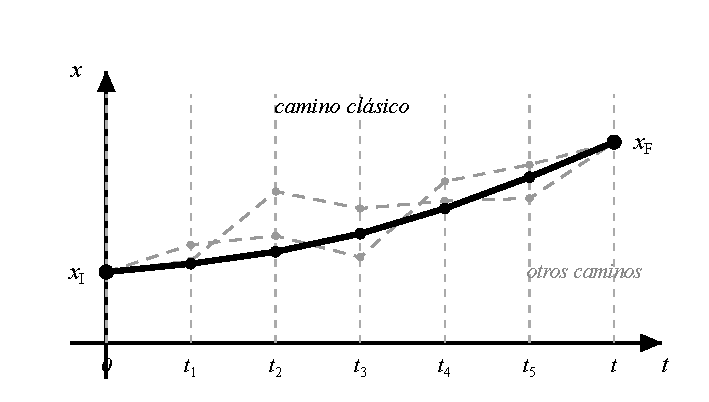
\includegraphics[width=0.66\linewidth]{Capitulo 3/Figuras/IntegralCamino.pdf}
            \caption{Construcción de la integral de camino. El intervalo se divide en rodajas y se integra sobre todas las posiciones intermedias posibles, de manera que a la amplitud contribuyen por igual el camino clásico y todos los caminos quebrados que lo rodean.}
            \label{fig:IntegralCamino}
        \end{figure}

        Sustituyendo \eqref{eq:EslabonFinal} en \eqref{eq:PropagadorRodajas}, el producto de exponenciales se convierte en la exponencial de la suma, y esa suma es una suma de Riemann que en el límite $N\rightarrow\infty$ tiende a la integral de la acción a lo largo del camino poligonal definido por los puntos intermedios,
        \begin{equation}\label{eq:SumaRiemann}
            \sum_{j=0}^{N-1}\varepsilon\left[\frac{m}{2}\left(\frac{x_{j+1}-x_{j}}{\varepsilon}\right)^{2} - V(x_{j})\right]
            \;\xrightarrow[N\rightarrow\infty]{}\;
            \int_{0}^{t}L\left(x,\dot{x}\right)ds = S[x] .
        \end{equation}
        Obtenemos finalmente la \textit{integral de camino de Feynman},
        \begin{equation}\label{eq:IntegralCamino}
            \boxed{\;K(x_{F},t;x_{I},0) = \int_{x(0)=x_{I}}^{x(t)=x_{F}}\mathcal{D}[x(s)]\;\exp\left\{\frac{i}{\hbar}S[x(s)]\right\},\;}
        \end{equation}
        donde el símbolo $\mathcal{D}[x(s)]$ abrevia el límite del producto de integrales sobre los puntos intermedios junto con los factores de normalización,
        \begin{equation}\label{eq:MedidaFeynman}
            \mathcal{D}[x(s)] = \lim_{N\rightarrow\infty}\left(\frac{m}{2\pi i\hbar\varepsilon}\right)^{N/2}\prod_{j=1}^{N-1}dx_{j} .
        \end{equation}

        El significado de \eqref{eq:IntegralCamino} es el que anunciamos al comienzo del capítulo. La amplitud de que la partícula vaya de un punto a otro es la suma de las contribuciones de \textit{todos} los caminos concebibles que los unen, sin excepción, incluidos los que violan groseramente las ecuaciones de movimiento, y cada camino contribuye con el mismo módulo y una fase igual a su acción medida en unidades de $\hbar$. La trayectoria clásica no tiene ningún privilegio a priori; adquiere su privilegio únicamente en el límite en que la acción típica es grande frente a $\hbar$, porque entonces las fases de caminos vecinos oscilan tan rápidamente que sus contribuciones se cancelan entre sí, salvo en la vecindad de aquel camino para el cual la acción es estacionaria y las fases vecinas coinciden en primer orden. \textbf{El principio de Hamilton deja así de ser un postulado y se convierte en el resultado de una interferencia}, y la objeción que se le hizo a Fermat en el siglo XVII, la de que la luz parecía necesitar conocer su destino, queda respondida: la luz no escoge, interfiere.

    \subsection{El propagador del oscilador armónico}

        Aplicaremos ahora el resultado al sistema que nos interesa. Para lagrangianos cuadráticos, como el del oscilador armónico \eqref{eq:LagrangianoOsc}, la integral de camino puede evaluarse exactamente, y el procedimiento consiste en separar cada camino en la trayectoria clásica más una desviación,
        \begin{equation}\label{eq:SeparacionCaminos}
            x(s) = x_{\mathrm{cl}}(s) + y(s), \qquad y(0) = y(t) = 0,
        \end{equation}
        donde la desviación se anula en los extremos porque todos los caminos comparten los mismos puntos inicial y final. Desarrollando la acción en potencias de $y$, y teniendo en cuenta que el término lineal se anula idénticamente porque la acción es estacionaria sobre $x_{\mathrm{cl}}$, que es precisamente lo que afirma el principio de Hamilton, y que para un lagrangiano cuadrático la serie se corta en el segundo orden,
        \begin{equation}\label{eq:AccionSeparada}
            S[x] = S_{\mathrm{cl}} + \textcolor{red}{\left.\frac{\delta S}{\delta x}\right|_{x_{\mathrm{cl}}}\!\!\cdot y} + \frac{1}{2}\left.\frac{\delta^{2}S}{\delta x^{2}}\right|_{x_{\mathrm{cl}}}\!\!\cdot y^{2}
            = S_{\mathrm{cl}} + \int_{0}^{t}\left(\frac{m}{2}\dot{y}^{2} - \frac{m\omega^{2}}{2}y^{2}\right)ds,
        \end{equation}
        donde el término marcado en rojo se anula por la estacionariedad. El factor $e^{iS_{\mathrm{cl}}/\hbar}$ sale entonces fuera de la integral funcional, porque no depende del camino de integración, y lo que queda es una integral sobre desviaciones con extremos nulos que no depende de $x_{I}$ ni de $x_{F}$ sino solo del tiempo transcurrido,
        \begin{equation}\label{eq:PropagadorFactorizado}
            K(x_{F},t;x_{I},0) = F(t)\,\exp\left[\frac{i}{\hbar}S_{\mathrm{cl}}(x_{F},t;x_{I},0)\right] .
        \end{equation}
        La evaluación del prefactor $F(t)$ exige calcular el determinante del operador de fluctuaciones, cálculo que no reproduciremos aquí y cuyo resultado, obtenido por primera vez por Van Vleck en el contexto del principio de correspondencia \citep{vanvleck1928correspondence}, es
        \begin{equation}\label{eq:VanVleck}
            F(t) = \left(\frac{1}{2\pi i\hbar}\,\frac{\partial^{2}S_{\mathrm{cl}}}{\partial x_{I}\,\partial x_{F}}\right)^{1/2} .
        \end{equation}

        Podemos ahora ensamblar el resultado para el oscilador. La acción clásica la calculamos en \eqref{eq:AccionOscilador}, y su derivada cruzada se obtiene derivando esa expresión primero respecto de $q_{I}$ y luego respecto de $q_{F}$: el único término que sobrevive a las dos derivaciones es el producto cruzado, pues los cuadrados desaparecen al derivar respecto de la otra variable,
        \begin{equation}\label{eq:DerivadaCruzada}
            \frac{\partial^{2}S_{\mathrm{cl}}}{\partial q_{I}\,\partial q_{F}}
            = \frac{\partial}{\partial q_{F}}\left[\frac{m\omega}{2\sin\omega t}\left(2q_{I}\cos\omega t - 2q_{F}\right)\right]
            = -\frac{m\omega}{\sin\omega t} .
        \end{equation}
        Sustituyendo \eqref{eq:DerivadaCruzada} en \eqref{eq:VanVleck} y absorbiendo el signo en la determinación de la raíz, el prefactor resulta ser $\left(m\omega/2\pi i\hbar\sin\omega t\right)^{1/2}$, de manera que el propagador completo es
        \begin{equation}\label{eq:PropagadorOscilador}
            \boxed{\;K(q_{F},t;q_{I},0) = \left(\frac{m\omega}{2\pi i\hbar\sin\omega t}\right)^{1/2}
            \exp\left\{\frac{i\,m\omega}{2\hbar}\left[\left(q_{I}^{2}+q_{F}^{2}\right)\cot\omega t - \frac{2q_{I}q_{F}}{\sin\omega t}\right]\right\} .\;}
        \end{equation}

        Esta expresión es el punto de llegada del capítulo y el punto de partida de los dos siguientes. La conexión, dicha explícitamente, es la siguiente. Cuando en el capítulo dedicado a la cuantización del campo electromagnético escribamos el hamiltoniano de cada modo en la forma $H = \frac{1}{2}\left(P^{2}+\omega^{2}Q^{2}\right)$, las variables canónicas estarán normalizadas de manera que la masa efectiva sea la unidad, y entonces \eqref{eq:PropagadorOscilador} se reduce a
        \begin{equation}\label{eq:PropagadorFoton}
            K(q_{F},t;q_{I},0) = \left(\frac{\omega}{2\pi i\hbar\sin\omega t}\right)^{1/2}
            \exp\left\{\frac{i\,\omega}{2\hbar}\left[\left(q_{I}^{2}+q_{F}^{2}\right)\cot\omega t - \frac{2q_{I}q_{F}}{\sin\omega t}\right]\right\},
        \end{equation}
        que es literalmente la amplitud de transición de la que parte el capítulo dedicado a la propagación fundamental de los fotones. \textbf{El propagador del fotón no es, por tanto, un postulado de la óptica cuántica sino la exponencial de la acción clásica de un oscilador armónico, calculada en \eqref{eq:AccionOscilador} sin más herramienta que las ecuaciones de Lagrange.}

        Y hay todavía una observación que merece hacerse, porque cierra el arco completo de estos apuntes. La estructura del exponente de \eqref{eq:PropagadorFoton}, una cotangente multiplicando la suma de los cuadrados y una cosecante multiplicando el producto cruzado, es exactamente la del núcleo de la transformada fraccionaria de Fourier que obtuvimos en el capítulo primero al estudiar la propagación de Fresnel entre dos esferas de referencia, con el ángulo fraccionario $\alpha$ desempeñando el papel de $\omega t$. La difracción de una onda luminosa clásica a lo largo de una distancia $z$ y la evolución temporal de un modo del campo cuantizado durante un tiempo $t$ son, en el plano formal, la misma transformación aplicada a objetos distintos. Esa coincidencia, que a estas alturas ya no puede sorprendernos, es la razón por la cual la óptica y la mecánica cuántica hablan el mismo idioma, y la analogía que Hamilton escribió en 1834 sigue produciendo resultados casi dos siglos después.
